%%%%%%%%%%%%%%%%%%%%%%%%%%%%%%%%%%%%%%%%%
% Wenneker Article
% LaTeX Template
% Version 2.0 (28/2/17)
%
% This template was downloaded from:
% http://www.LaTeXTemplates.com
%
% Authors:
% Vel (vel@LaTeXTemplates.com)
% Frits Wenneker
%
% License:
% CC BY-NC-SA 3.0 (http://creativecommons.org/licenses/by-nc-sa/3.0/)
%
%%%%%%%%%%%%%%%%%%%%%%%%%%%%%%%%%%%%%%%%%

%----------------------------------------------------------------------------------------
%	PACKAGES AND OTHER DOCUMENT CONFIGURATIONS
%----------------------------------------------------------------------------------------

\documentclass[12pt, a4paper]{article} % 10pt font size (11 and 12 also possible), A4 paper (letterpaper for US letter) and two column layout (remove for one column)

\usepackage[english]{babel} % English language hyphenation
\usepackage{microtype} % Better typography
\usepackage{amsmath,amsfonts,amsthm} % Math packages for equations
\usepackage[svgnames]{xcolor} % Enabling colors by their 'svgnames'
\usepackage[hang, small, labelfont=bf, up, textfont=it]{caption} % Custom captions under/above tables and figures
\usepackage{booktabs} % Horizontal rules in tables
\usepackage{lastpage} % Used to determine the number of pages in the document (for "Page X of Total")
\usepackage{graphicx} % Required for adding images
\usepackage{amssymb}
\usepackage[mathscr]{eucal}
\usepackage[table]{xcolor}
\usepackage{enumitem} % Required for customising lists
\setlist{noitemsep} % Remove spacing between bullet/numbered list elements
\usepackage{sectsty} % Enables custom section titles
\allsectionsfont{\usefont{OT1}{phv}{b}{n}} % Change the font of all section commands (Helvetica)
\usepackage{hyperref}
\usepackage[sort,numbers]{natbib}
\usepackage{fancyhdr}
\usepackage{verbatim} 
%----------------------------------------------------------------------------------------
%	MARGINS AND SPACING
%----------------------------------------------------------------------------------------
\usepackage{geometry} % Required for adjusting page dimensions
\geometry{
	top=0.65cm, % Top margin
	bottom=1.5cm, % Bottom margin
	left=1.5cm, % Left margin
	right=1.5cm, % Right margin
	includehead, % Include space for a header
	includefoot, % Include space for a footer
	%showframe, % Uncomment to show how the type block is set on the page
}
\setlength{\columnsep}{6mm} % Column separation width

%----------------------------------------------------------------------------------------
%	FONTS
%----------------------------------------------------------------------------------------

\usepackage[T1]{fontenc} % Output font encoding for international characters
\usepackage[utf8]{inputenc} % Required for inputting international characters
\usepackage{XCharter} % Use the XCharter font
\pagestyle{headings}

%%%%%%%%%%%%%%%%%%%%%%%%%%%%%%%%%%%%%%%%%%
% Wenneker Article
% Structure Specification File
% Version 1.0 (28/2/17)
%
% This file originates from:
% http://www.LaTeXTemplates.com
%
% Authors:
% Frits Wenneker
% Vel (vel@LaTeXTemplates.com)
%
% License:
% CC BY-NC-SA 3.0 (http://creativecommons.org/licenses/by-nc-sa/3.0/)
%
%%%%%%%%%%%%%%%%%%%%%%%%%%%%%%%%%%%%%%%%%

%----------------------------------------------------------------------------------------
%	PACKAGES AND OTHER DOCUMENT CONFIGURATIONS
%----------------------------------------------------------------------------------------

\usepackage[english]{babel} % English language hyphenation

\usepackage{microtype} % Better typography

\usepackage{amsmath,amsfonts,amsthm} % Math packages for equations

\usepackage[svgnames]{xcolor} % Enabling colors by their 'svgnames'

\usepackage[hang, small, labelfont=bf, up, textfont=it]{caption} % Custom captions under/above tables and figures

\usepackage{booktabs} % Horizontal rules in tables

\usepackage{lastpage} % Used to determine the number of pages in the document (for "Page X of Total")

\usepackage{graphicx} % Required for adding images

\usepackage{enumitem} % Required for customising lists
\setlist{noitemsep} % Remove spacing between bullet/numbered list elements

\usepackage{sectsty} % Enables custom section titles
\allsectionsfont{\usefont{OT1}{phv}{b}{n}} % Change the font of all section commands (Helvetica)

%----------------------------------------------------------------------------------------
%	MARGINS AND SPACING
%----------------------------------------------------------------------------------------

\usepackage{geometry} % Required for adjusting page dimensions

\geometry{
	top=1cm, % Top margin
	bottom=1.5cm, % Bottom margin
	left=2cm, % Left margin
	right=2cm, % Right margin
	includehead, % Include space for a header
	includefoot, % Include space for a footer
	%showframe, % Uncomment to show how the type block is set on the page
}

\setlength{\columnsep}{7mm} % Column separation width

%----------------------------------------------------------------------------------------
%	FONTS
%----------------------------------------------------------------------------------------

\usepackage[T1]{fontenc} % Output font encoding for international characters
\usepackage[utf8]{inputenc} % Required for inputting international characters

\usepackage{XCharter} % Use the XCharter font

%----------------------------------------------------------------------------------------
%	HEADERS AND FOOTERS
%----------------------------------------------------------------------------------------

\usepackage{fancyhdr} % Needed to define custom headers/footers
\pagestyle{fancy} % Enables the custom headers/footers

\renewcommand{\headrulewidth}{0.0pt} % No header rule
\renewcommand{\footrulewidth}{0.4pt} % Thin footer rule

\renewcommand{\sectionmark}[1]{\markboth{#1}{}} % Removes the section number from the header when \leftmark is used

%\nouppercase\leftmark % Add this to one of the lines below if you want a section title in the header/footer

% Headers
\lhead{} % Left header
\chead{\textit{\thetitle}} % Center header - currently printing the article title
\rhead{} % Right header

% Footers
\lfoot{} % Left footer
\cfoot{} % Center footer
\rfoot{\footnotesize Page \thepage\ of \pageref{LastPage}} % Right footer, "Page 1 of 2"

\fancypagestyle{firstpage}{ % Page style for the first page with the title
	\fancyhf{}
	\renewcommand{\footrulewidth}{0pt} % Suppress footer rule
}

%----------------------------------------------------------------------------------------
%	TITLE SECTION
%----------------------------------------------------------------------------------------

\newcommand{\authorstyle}[1]{{\large\usefont{OT1}{phv}{b}{n}\color{DarkRed}#1}} % Authors style (Helvetica)

\newcommand{\institution}[1]{{\footnotesize\usefont{OT1}{phv}{m}{sl}\color{Black}#1}} % Institutions style (Helvetica)

\usepackage{titling} % Allows custom title configuration

\newcommand{\HorRule}{\color{DarkGoldenrod}\rule{\linewidth}{1pt}} % Defines the gold horizontal rule around the title

\pretitle{
	\vspace{-30pt} % Move the entire title section up
	\HorRule\vspace{10pt} % Horizontal rule before the title
	\fontsize{32}{36}\usefont{OT1}{phv}{b}{n}\selectfont % Helvetica
	\color{DarkRed} % Text colour for the title and author(s)
}

\posttitle{\par\vskip 15pt} % Whitespace under the title

\preauthor{} % Anything that will appear before \author is printed

\postauthor{ % Anything that will appear after \author is printed
	\vspace{10pt} % Space before the rule
	\par\HorRule % Horizontal rule after the title
	\vspace{20pt} % Space after the title section
}

%----------------------------------------------------------------------------------------
%	ABSTRACT
%----------------------------------------------------------------------------------------

\usepackage{lettrine} % Package to accentuate the first letter of the text (lettrine)
\usepackage{fix-cm}	% Fixes the height of the lettrine

\newcommand{\initial}[1]{ % Defines the command and style for the lettrine
	\lettrine[lines=3,findent=4pt,nindent=0pt]{% Lettrine takes up 3 lines, the text to the right of it is indented 4pt and further indenting of lines 2+ is stopped
		\color{DarkGoldenrod}% Lettrine colour
		{#1}% The letter
	}{}%
}

\usepackage{xstring} % Required for string manipulation

\newcommand{\lettrineabstract}[1]{
	\StrLeft{#1}{1}[\firstletter] % Capture the first letter of the abstract for the lettrine
	\initial{\firstletter}\textbf{\StrGobbleLeft{#1}{1}} % Print the abstract with the first letter as a lettrine and the rest in bold
}

%----------------------------------------------------------------------------------------
%	BIBLIOGRAPHY
%----------------------------------------------------------------------------------------

\usepackage[backend=bibtex,style=authoryear,natbib=true]{biblatex} % Use the bibtex backend with the authoryear citation style (which resembles APA)

\addbibresource{example.bib} % The filename of the bibliography

\usepackage[autostyle=true]{csquotes} % Required to generate language-dependent quotes in the bibliography
 % Specifies the document structure and loads requires packages

%----------------------------------------------------------------------------------------
%	ARTICLE INFORMATION
%----------------------------------------------------------------------------------------
\begin{document}
\pagestyle{fancy}
\fancyhf{}
%\fancyhead[LE,RO]{Overleaf}
%\fancyhead[RE,LO]{Guides and tutorials}
\fancyfoot[LO,RE]{FETOPEN-01 template WP18-20 v20171106}
\fancyfoot[LE,RO]{$\mathcal{ROBHOOT}$}


\title{$\mathcal{ROBHOOT}$ \\ Open Discovery Network \\ FET v.1.0}} % The article title
  %\author{{\textsuperscript{1,2,3} and XY\textsuperscript{2,3}}% Authors
  \newline\newline % Space before institutions
  \\
%	\textsuperscript{1}\institution{}\\ % Institution 1
%	\textsuperscript{2}\institution{}\\ % Institution 2
	%\textsuperscript{3}\institution{\texttt{LaTeXTemplates.com}}
      %} % Institution 3


% Example of a one line author/institution relationship
%\author{\newauthor{John Marston} \newinstitution{Universidad Nacional Autónoma de México, Mexico City, Mexico}}

\date{\today} % Add a date here if you would like one to appear underneath the title block, use \today for the current date, leave empty for no date
%---------------------------------------------------------------------------------------

\maketitle % Print the title
%\thispagestyle{firstpage} % Apply the page style for the first page (no headers and footers)

%----------------------------------------------------------------------------------------
%	ABSTRACT
%----------------------------------------------------------------------------------------
\section{{\bf Summary}} Global sustainability is a
  major goal of humanity. Many studies have shown global
  sustainability could be achieved by strengthening transparency and
  feedbacks between social, ecological, technological and governance
  systems. Sustainability goals, however, strongly depend on global
  access to evidence- and research-based knowledge gaps. Yet, the
  science ecosystem lacks open-source technologies narrow down
  knowledge gaps. We introduce an open discovery network targeting
  knowledge gaps throughout open-access generation of fully
  reproducible science reports. Open discovery network encompasses a
  hybrid-automated-technology to lay out the foundation of an
  open-science ecosytem strengthening the robustness,
  decentralization, reproducibility and social accessibility of
  science. The project summarized here is not set out to deliver a
  finished open discovery network, but to provide the architecture of
  a science-enabled technology as a proof-of-principle to connect
  decentralized and neutral-knowledge generation with
  knowledge-inspired societies.
%----------------------------------------------------------------------------------------
%	ARTICLE CONTENTS
% ----------------------------------------------------------------------------------------
\section{Excellence}
\subsection{Radical vision of a science-enabled technology}
We are in the midst of the fourth industrial revolution, a
transformation revolving around data driven intelligent machines. Yet,
despite the rapid evolution of the digital ecosystem around data
driven intelligent machines, open discovery-based technologies
facilitating global access to informed decisions when solving complex
social, environmental and technological problems are particularly
lacking. How can discovery driven intelligent machines help to reach global
sustainability goals by reducing knowledge gaps? The
$\mathcal{ROBHOOT}$ project introduces new concepts to global
knowledge gaps. Current technologies for automated scientific inquiry
are highly fragmented, partly solve reproducibility and are mostly
developed in close-source software. Thus, despite the importance of
global access to knowledge gaps for reaching sustainability goals,
open-source technologies fully accounting for the research cycle to
generate reproducible science reports are lacking. The goal of
$\mathcal{ROBHOOT}$ is to propose a new hybrid-technology concept
combining question- and reproducibility-based decentralized
knowledge-graphs to lay the foundation for a novel, global access to
scientific discovery technology.



ontain multiple steps of information transfer
among trusted and untrusted peers. As a consequence, science generates
knowledge with specific features. Which are the desirable features of
human-generated knowledge? Should such features be aligned with taking
informed decisions in complex social, governance, environmental and
technological problems? Can global transparency in knowledge
generation be achieved to facilitate sustainability goals of humanity?
Currently public funded science is highly centralized
\citep{Inhaber1977,Gunther2018}⁠⁠, prone to errors \citep{Fang2011},
difficult to reproduce \citep{Hardwicke2018}, and contains many biases
\citep{Ioannidis2005}. This makes science an ecosystem building up
problems to decrease the evidence- and research-based knowledge gaps
in humanity \citep{Mastrangelo2019}. Here we propose an open research
network fully accounting for the research cycle. The goal of such a
technology is to reduce global knowledge gaps while accounting for
centralization, bias, error-prone, non-reproducibility and lack of
incentives in the existing science and technology ecosystem (Figure 1
and Table 1).

%\begin{figure}
%  \centering
%  \hspace{-0.25 in}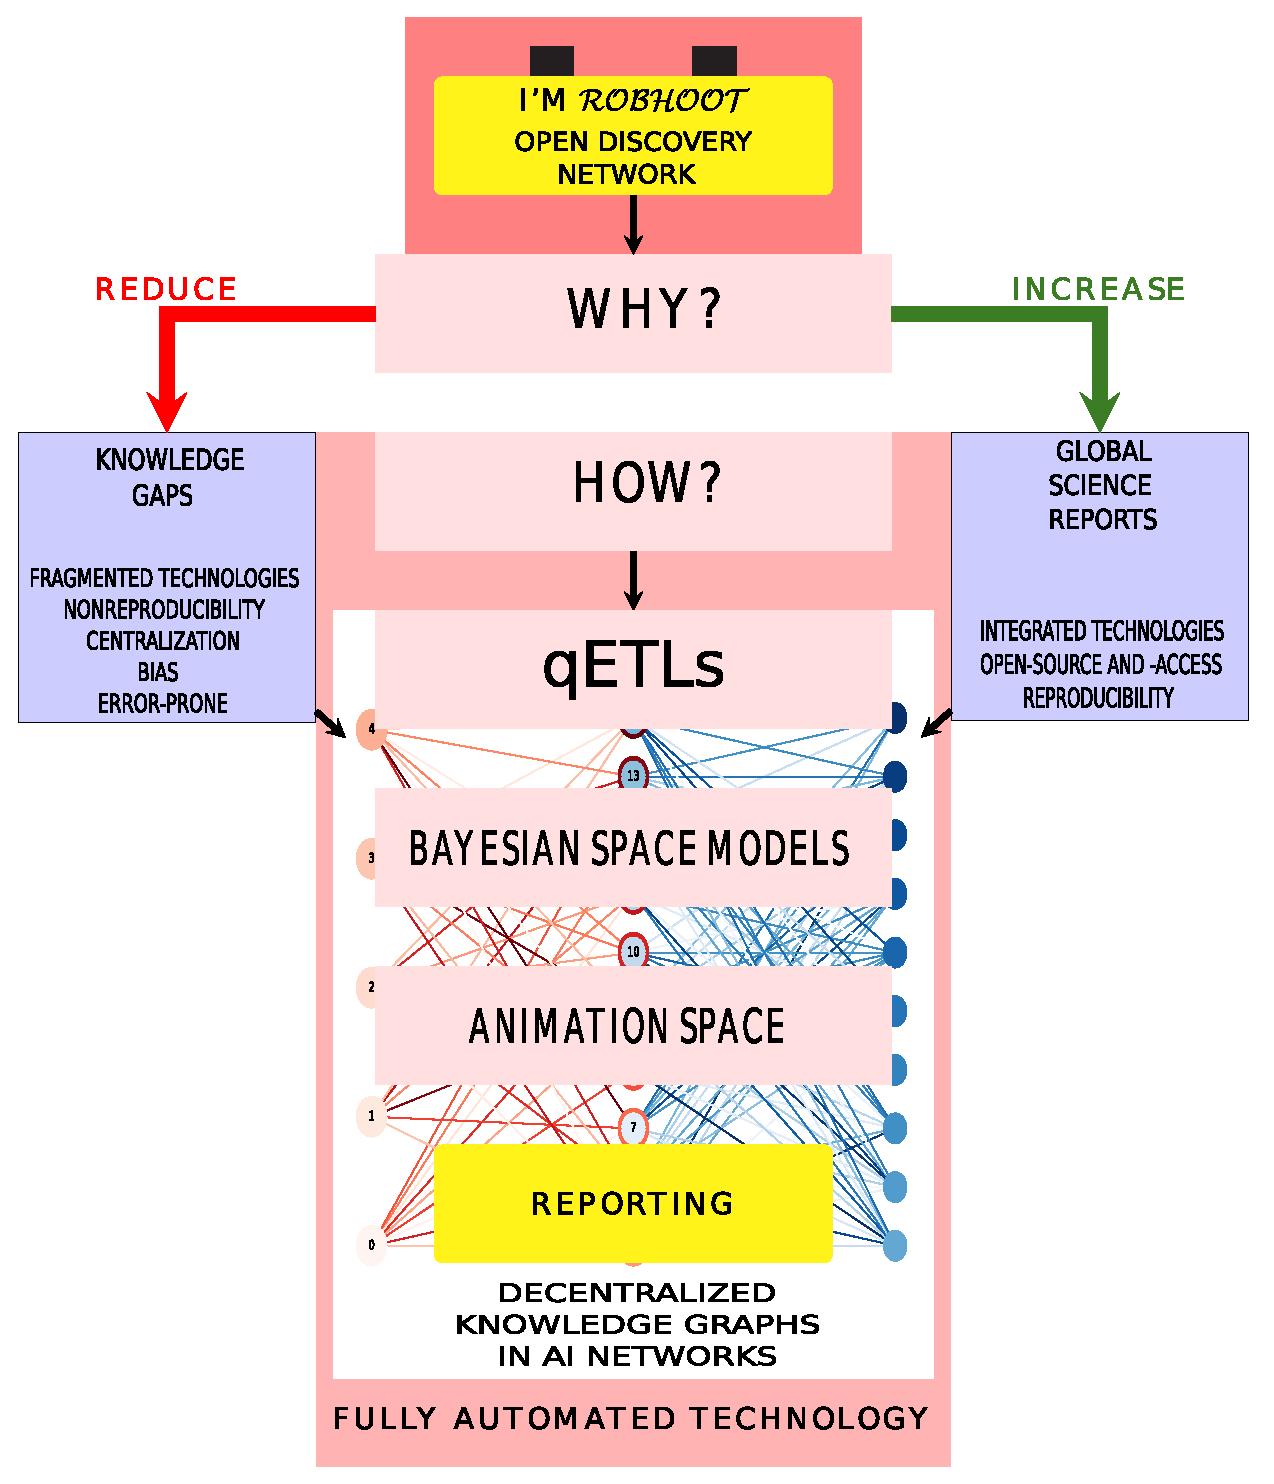
\includegraphics[width=0.65\textwidth]{flowchart.pdf}
%  \small {\bf Figure 1: Open discovery network technology}. {\bf
%    $\mathcal{ROBHOOT}$} targets global knowledge gaps (red path) and
%  open-access fully reproducible discovery reports (green
%  path). $\mathcal{ROBHOOT}$ is open-source science-based automated
%  technology decentralizing reproducible knowledge
%  graphs. $\mathcal{ROBHOOT}$} integrates 1) question-based knowledge
%gaps with data extraction, transformation and loading algorithms for
%database integration and complexity reduction ({\bf qETLs}), 2) {\bf
%  Bayesian Space Models} accounting for open-ended model optimization
%techniques, 3) {\bf Animation Space} visualizing fitting procedures
%and pattern generation connecting empirical data and open-ended
%models, and 4) open and globally accessible {\bf Reporting} formalized
%in natural processing language.}
%\end{figure}

\begin{figure}
  %\begin{minipage}[c]{0.75\textwidth}
    \hspace{-0.25 in}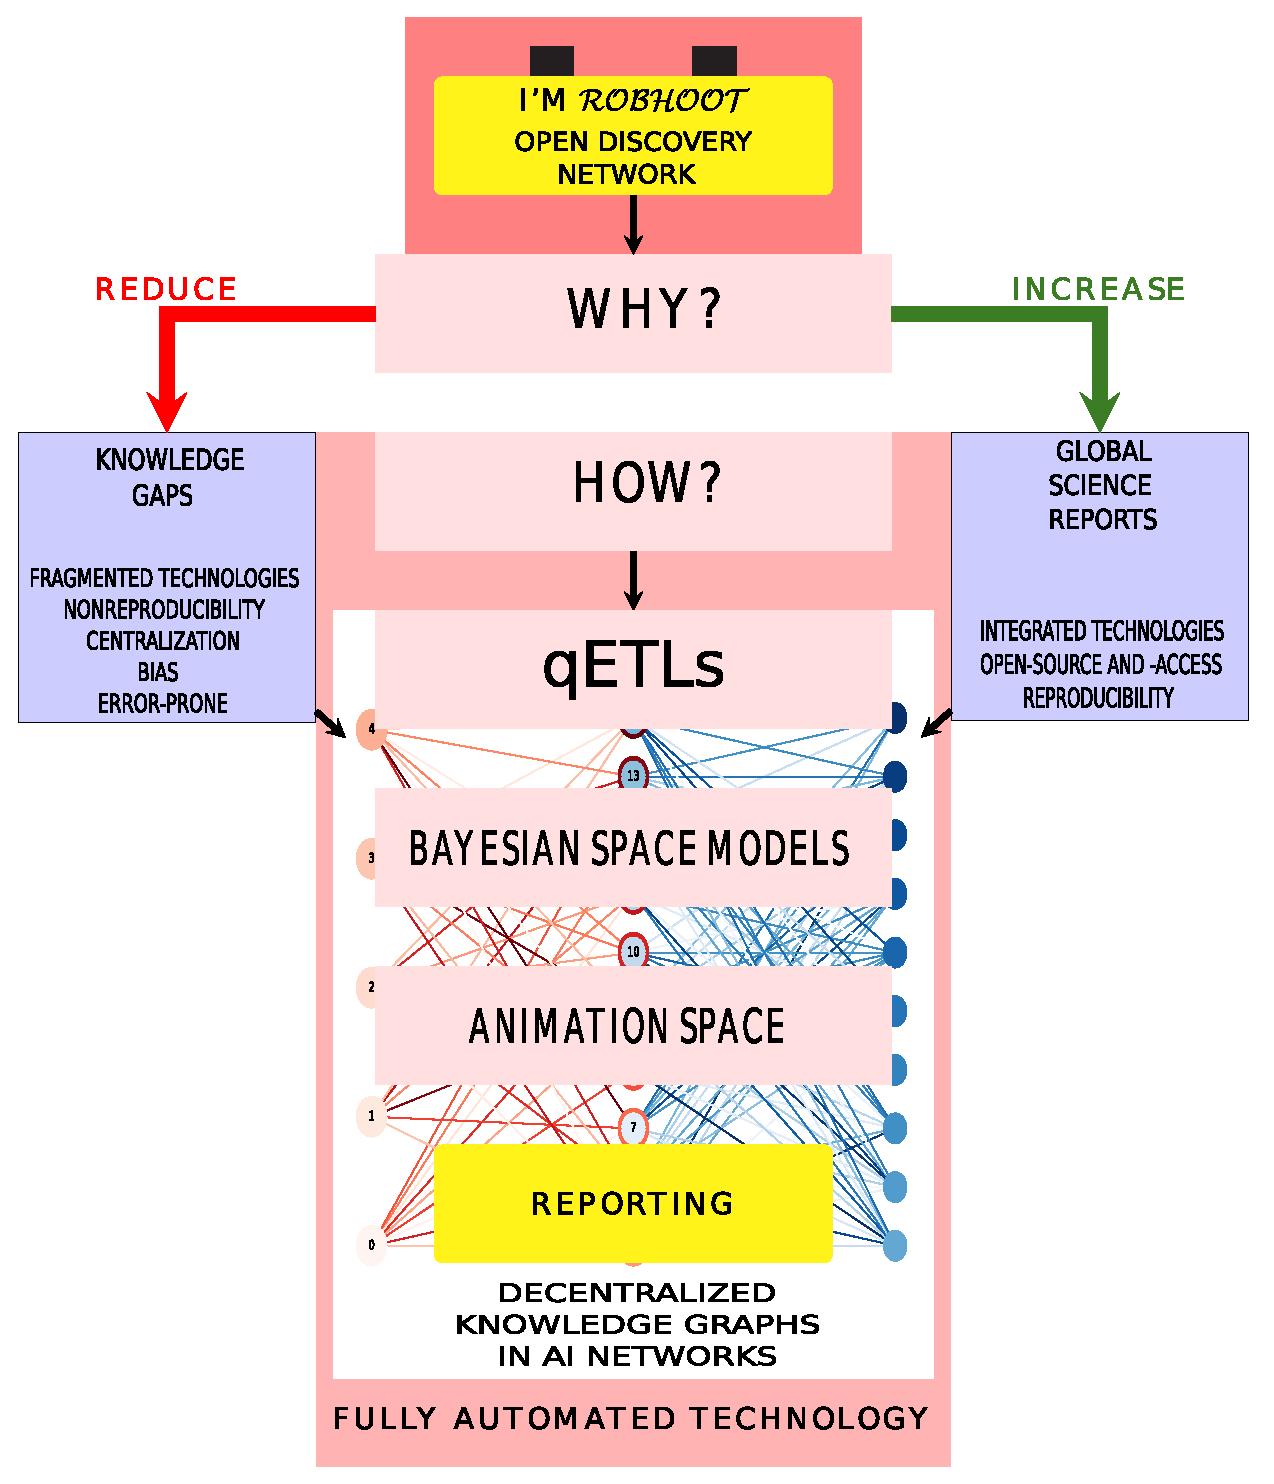
\includegraphics[width=0.65\textwidth]{flowchart.pdf}
  %\end{minipage}\hfill
  %\begin{minipage}[c]{0.5\textwidth}
    \caption*{\small {\bf Figure 1: Open discovery network
        technology}. $\mathcal{ROBHOOT}$ targets global knowledge gaps
      (red path) and open-access fully reproducible discovery reports
      (green path). $\mathcal{ROBHOOT}$ is open-source science-based
      automated technology decentralizing reproducible knowledge
      graphs. $\mathcal{ROBHOOT}$ integrates 1) question-based
      knowledge gaps with data extraction, transformation and loading
      algorithms for database integration and complexity reduction
      ({\bf qETLs}), 2) {\bf Bayesian Space Models} accounting for
      open-ended model optimization techniques, 3) {\bf Animation
        Space} visualizing fitting procedures and pattern generation
      connecting empirical data and open-ended models, and 4) open and
      globally accessible {\bf Reporting} formalized in natural
      processing language.}}
  %\end{minipage}
\end{figure}


\begin{comment}
  The Robhoot project is trying to introduce new concepts to allow
  scientist and the public to interact in a decentralized open-access
  knowledge network to gain informed decisions when solving complex
  social, environmental and technological problems. Current
  technologies for scientific inquiry are highly fragmented and thus
  only increase robustness, reproducibility and the interactions with
  the public marginally (refs). The goal of Robhoot is to propose a
  new hybrid-technology concept combining deep learning, automation
  and distributed ledger technology with the advances of neural
  biological networks to lay the foundation for a novel open-science
  ecosystem aiming to couple predictive and knowledge power in
  contemporary societies. Robhoot is not set out to deliver a finished
  deep knowledge ledger network in the science ecosystem but provide a
  science-enabled technology in establishing a prototype
  proof-of-principle for an open public-science ecosystem.
  \end{comment}

 
\begin{table}
 %\rowcolor{pink}
\begin{tabular}{ p{6cm} | p{3cm} | p{3cm}}
  \hline \hline
  \textbf{Features} & \textbf{Science Ecosystem} &\textbf{{\bf $\mathcal{ROBHOOT}$}}\\  \hline
  Decentralization & No & Yes \\ \hline
  Full automation & No & Yes \\ \hline
  Open-access & Mostly No & Yes \\ \hline
  Immutability & No & Yes \\ \hline
  Robustness & Mostly No & Yes \\ \hline
  Reproducibility & Mostly No & Yes \\ \hline        
  Owner-Controlled assets & No & Yes \\ \hline       
  \bottomrule
\end{tabular}
\caption{{\bf $\mathcal{ROBHOOT}$} is designed to resolve desirable
  properties of science: Open-access, immutability, robustness,
  reproducibility, and owner-controlled assets. These features will be
  added during the different stages of development of the project
  (section ``Design Goals'').}
\end{table}
The core feature of an open research network is to embed
knowledge-generation into reproducible automation and
decentralization. Currently, many studies focusing on decentralized
ecosystems are producing an immense gain of knowledge in a variety of
sectors about scalability, security and decentralization trade-offs
\citep{Golem2016,Durov2017,Androulaki2018,OceanProtocolFoundation2018,BigchainDBGmbH2018}. In
the open science ecosystem, only a few implementations of
decentralized technologies exist \citep{Gunther2018}. Automation and
AI technologies represent the other angle from which many advances are
rapidly occurring in digital ecosystems
\citep{Schmidhuber:2015,Reichstein,Gil2019}. While the existing
technological paradigm in many sectors is rapidly shifting towards
science-based decentralization and automation technologies, the
science ecosystem currently lack decentralized, neutral and
open-source knowledge-inspired technologies strongly impacting
knowledge-inspired societies (Figure 1 and Tables 1 to 3). Rapid
advances of research platforms automating parts of the research cycle
are currently under development
\citep{Steinruecken,Guimera}.\footnote{This is by no means an
  exhaustive list but it gives an indication of the many projects
  currently in place:
  \href{https://www.nterminal.com}{NakamotoT},\href{https://cloud.google.com/bigquery/}{BigQuery},\href{https://www.automaticstatistician.com/index/}{Automated
    statistician},\href{http://www.modulos.ai/}{Modulos},\href{https://ai.google/}{Google
    AI},\href{https://iris.ai}{Iris},\href{https://github.com/DS3Lab/easeml}{easeml},\href{https://www.datarobot.com/}{datarobot},\href{https://aito.ai/}{aito},\href{https://www.nutonian.com/products/eureqa/}{eureqa}}
However, most of the existing research projects aiming to automate
part of the research cycle are being built around close-source
software. Therefore, open-source, reproducible, decentralized and
automated technologies accounting for the research cycle are at a very
incipient stage of development. To move forward open-source
technologies accounting for the research cycle we need to compactly
integrate knowledge-generation (Figure 2a) to automated tools
connecting knowledge graphs (Figure 2b) and deep learning networks
(Figure 2c) in fully decentralized ecosystems (Figure 2d).

\section{The objectives of the proposal}
The $\mathcal{ROBHOOT}$ consortium will build on the achievements of
many open-source software projects, the open-source digital ecosystem,
exploring novel features to reach a fully automated technology
targeting a global reduction of knowledge gaps. $\mathcal{ROBHOOT}$
proposes to go far beyond the existing partial solutions to
reproducibility and automation to track, understand and predict how
knowledge is made during the discovery process. $\mathcal{ROBHOOT}$
will build science-process understanding by making the full research
cycle reproducible.

It is a vision that can steer discovery into the future global access
of knowledge-inspired societies.

Many technologies at the center of
LifeTime are key European research strengths that the Flagship could
boost. These include single-cell technologies combined with advanced
imaging, artificial intelligence and patient-matched organoids, or
organ-on-a-chip disease models to study the progression of an illness
and develop novel therapeutics.



is set to be developed in four stages each with
one main goal (Figure 2). The most advanced version is to provide
open-access automated and fully reproducible reporting in a
decentralized network. $\mathcal{ROBHOOT}$ v.1.0} features an
automated research cycle connecting question generation to data
integration and reporting. {\bf b}) {\bf $\mathcal{ROBHOOT}$ v.2.0}
traces research paths as shown in {\bf a} using reproducible knowledge
graphs (KGs). {\bf c}) {\bf $\mathcal{ROBHOOT}$ v.3.0} contrasts deep
leaning networks to explore populations of KGs for gaining
undestanding of the process-based patterns contained in the data, and
{\bf d}) {\bf $\mathcal{ROBHOOT}$ v.4.0} deploys KGs in a
decentralized network of trusting/untrusting peers with every peer
maintaining the population of the KGs.

\section{How they will be achieved}


\begin{figure*}[ht]
  \vspace{-0.34 in}
    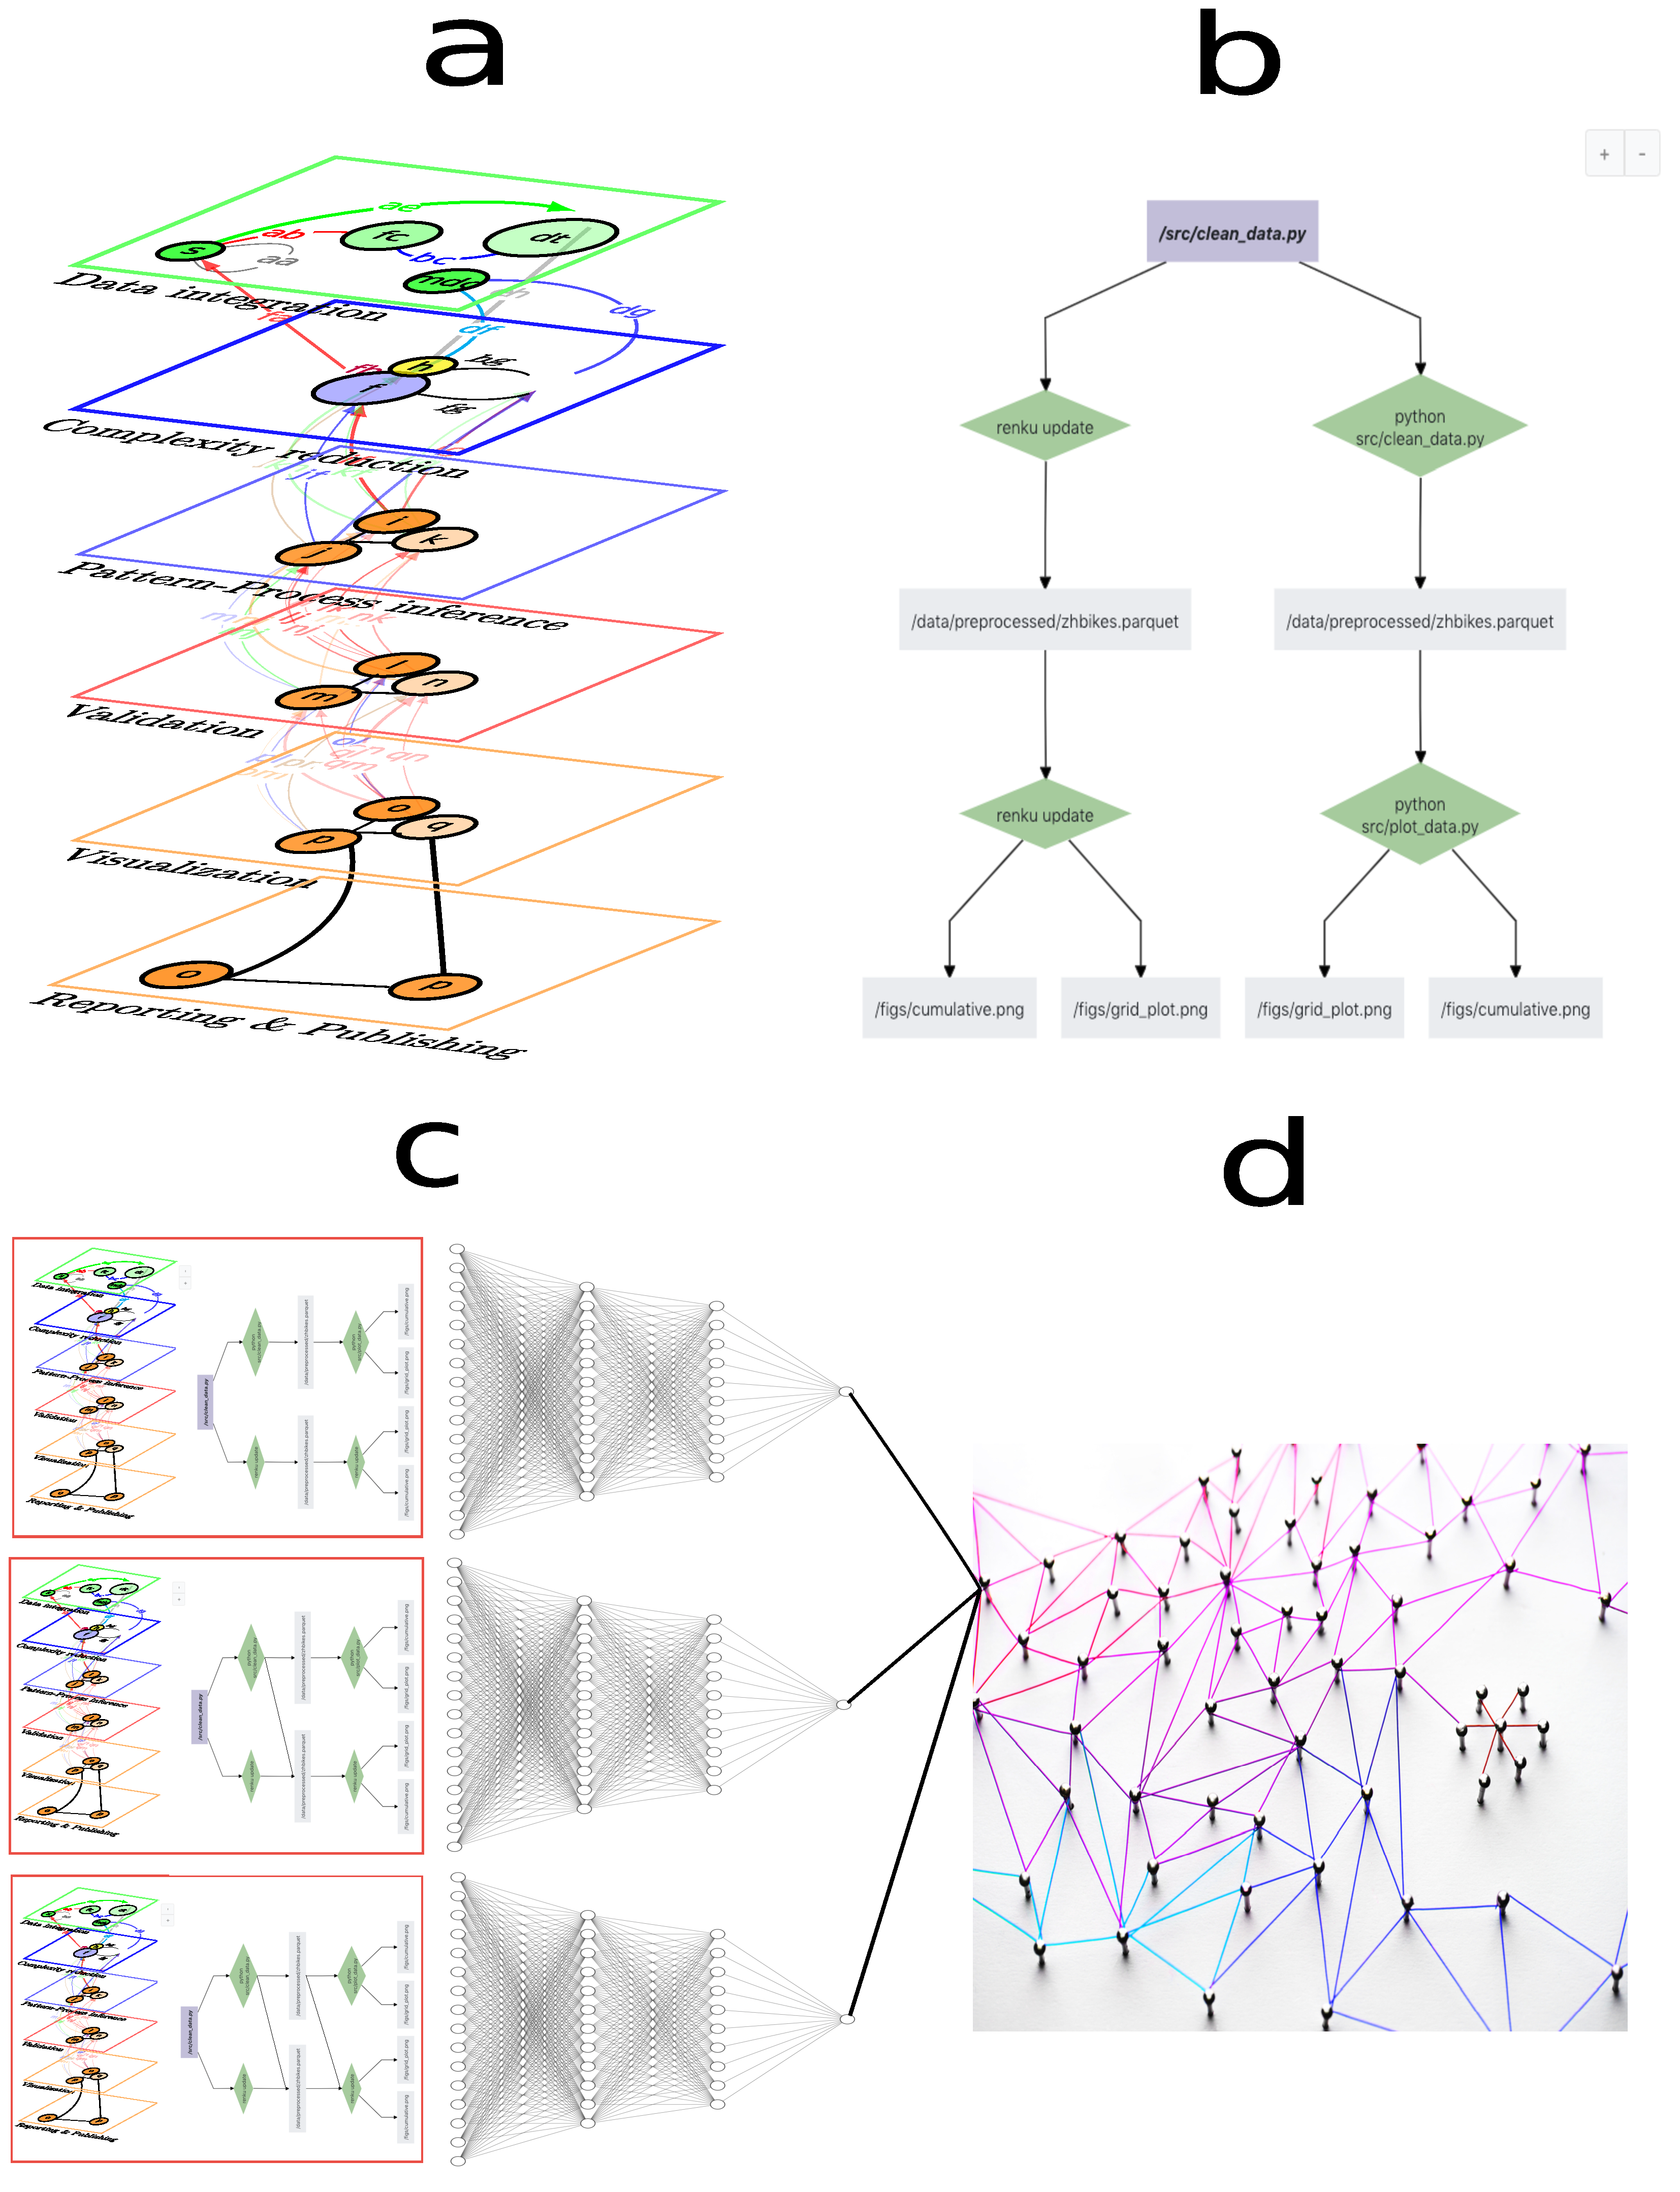
\includegraphics[width=14cm,height=15.5cm]{Figure1.pdf}
    \centering
    \caption{{\small {\bf Figure 2: How $\mathcal{ROBHOOT}$'s goals
          will be achieved?}. {\bf a}) {\bf $\mathcal{ROBHOOT}$ v.1.0}
        features an automated research cycle connecting question
        generation to data integration,inference, visualization and reporting. {\bf b}) {\bf
          $\mathcal{ROBHOOT}$ v.2.0} traces research paths as shown in
        {\bf a} using reproducible knowledge graphs (KGs). {\bf c})
        {\bf $\mathcal{ROBHOOT}$ v.3.0} contrasts deep leaning
        networks to explore populations of KGs for gaining
        undestanding of the process-based patterns contained in the
        data, and {\bf d}) {\bf $\mathcal{ROBHOOT}$ v.4.0} deploys KGs
        in a decentralized network of trusting/untrusting peers with
        every peer maintaining the population of the KGs.}
  \end{figure*}
    
      \begin{comment}
        Figure 1: Deep knowledge-based ledger network technology. a)
        End-to-end research from data integration to reporting. b) The
        knowledge graph (KG) representing one research path of a
        (i.e., Renku open-source code). c) Deep knowledge-based
        algorithms exploring the population of KGs to gain rule-based
        knowledge of the data. d) The population of all KGs is stored
        in a distributed ledger network of mutually
        trusting/untrusting peers with every peer maintaining the
        population of the KGs (i.e., decentralized P2P git network
        like Gitchain.) The end-to-end automated research connects
        citizen data science and open-science to knowledge-inspired
        societies in a integrated loop.}
      \end{comment}

      Mapping partly the discovery process is highly informative and
      challenging by itself, but a diverse group of X scientists
      across Europe decided that merely taking for reproducibility
      parts of the scientific process is not enough. Science is a
      highy dynamic process and there are many paths from where it can
      be achieved. To understand how discovery is generated, these
      scientists want to track the steps from questions to reporting
      and dissemination. To this end, they formed the
      $\mathcal{ROBHOOT}$ consortium with the goal of establishing an
      integrated toolbox containing several novel
      methods. $\mathcal{ROBHOOT}$ scientists will develop analytical
      and computational strategies such as machine-learning and
      artificial intelligence methods that help to understand
      discovery mechanisms and predict the future of global
      disemination of knowledge to science towards knowledge-inspired
      society. This strategy is expected to improve early access to
      discovery, predict the course of how science is evaluated and
      indentify new emerging targets where automation and global
      reports can play a key role in knowledge-inspired
      societies. $\mathcal{ROBHOOT}$'s goals will be developed in four
      different stages.

  \subsection{{\bf $\mathcal{ROBHOOT}$ v.1.0}: \\Automated Research Cycle}
  Discovery usually starts with an idea, and the research process is
  all about successfully bringing such an idea to the science
  ecosystem. and to the Algorithms detecting questions poorly explored
  but important for multidisciplinarity in the discovery process.

  \begin{itemize}
  \item {\bf Question generator} finds the weaknesses of question
    knowledge graphs to discover relevant topics across discipines.
  \item {\bf Universal ETLs} connects open-source generalized
    fault-tolerance algorithms connecting relevant questions to the
    extraction, transformation and load of data with unique features
    (i.e., formats, historical-real time, storage, dimensions, size,
    sampling bias and spatiotemporal resolution, etc) (Figures 1 and
    2a, two top layers).
   \item {\bf Bayesian space models} explore open-ended language of
     models combining Bayesian networks and optimization methods. The
     Bayesian space models module will search, evaluate models,
     trading-off complexity, fit to data and quantify resource usage
     (Figures 1 and 2a, inference and validation layers). 
   \item {\bf Animation Space} will connect open-source visualization
     software to the exploration of open-ended models to make the
     whole search transparent, highly visual and reproducible (Figures
     1 and 2a, visualization layer).
   \item {\bf Reporting} will develop a procedure to automatically
     explain the structure of the Bayesian space modeling module. It
     will also communicate the module using visualizations of the
     procedures followed by the Universal ETLs and Bayesian space
     models modules (Figures 1 and 2a, reporting layer).
   \item Robhoot 1.0 testnet is an automated reporting generation on
     ``Biodiversity, Global Change and Sustainability Research'' to
     explore the robustness of the automated research cycle accounting
     for {\bf Universal ETLs}, {\bf Bayesian space models}, {\bf
       Animation space} algorithms and {\bf Reporting} in natural
     processing languages.
   \end{itemize}

   \begin{itemize}
   \item {\bf Tools and Methods}: Multilayer networks metrics,
     Bayesian Networks, Julia, Python, Open-source software protocols,
     Gitchain, ETLs open-source software, Kafka, Clickhouse, Fluentd,
     Hadoop.
   \end{itemize}


   \begin{comment}
     Highlight case study more :: Data integrtaion of large scale
     models of species distributions
     https://onlinelibrary.wiley.com/doi/pdf/10.1111/j.1558-5646.2011.01265.x
   \end{comment}
     
    \begin{itemize}
    \item {\bf Novel territory}: Develop universal open-source ETLs
      algorithms and Bayesian space models and connect them to
      reporting automation in a ``Biodiversity, Global Change and
      Sustainability Research'' case study.
   \end{itemize}

   
\begin{table*}[ht]
 %\rowcolor{pink}
\begin{tabular}{ p{5.5cm} | p{11cm}}
  \hline \hline
  \textbf{Word} &\textbf{Meaning}\\  \hline
  Reproducible knowledge graph & Algorithms accounting for the research cycle to make it fully transparent\\ \hline
  Evidence-based knowledge gap & Factors limiting scientific transfer to benefit society\\ \hline
  Research-based knowledge gap & Factors limiting access to reproducibility in science\\ \hline
  Question-based knowledge graph & Algorithms detecting questions poorly explored but important for multidisciplinarity in science\\ \hline
  Automation & Functionally interdependent algorithms targeting minimal human-driven interference\\ \hline
  Knowledge-inspired society & Open access reproducible reports for global society \\ \hline
  Neutral-knowledge generation & Open reproducible reports accounting for the many biases of the scientiic process\\ \hline

  \bottomrule
\end{tabular}
\caption{{\bf Glossary of terms.}}
\end{table*}

   
  \subsection{{\bf $\mathcal{ROBHOOT}$ v.2.0}: \\ Reproducible Knowledge Graphs}
  \begin{itemize}
  \item Implementation of algorithms tracking paths of the research
    cycle with Reproducible Knowledge Graphs (KGs) (Figure 2b).
  \item Robustness and stability of searching and fitting procedures
    following a suite of open-source lineage client-tracker
    algorithms.
  \end{itemize}

   \begin{itemize}
   \item {\bf Tools and Methods}: Reproducible knowlegde graph
     algorithms and open-source packages (i.e., Renku and others).
   \end{itemize}

    \begin{itemize}
    \item {\bf Novel Territory}: Contrasting a set of Reproducible
      Knowledge Graphs algorithms to quantify the reproducibility,
      reusability, and recovery properties of the full research cycle.
   \end{itemize}

  %\vspace{-0.15 in}
  
  \subsection{{\bf $\mathcal{ROBHOOT}$ v.3.0}: \\ Deep learning networks}
  \begin{itemize}
  \item Deployment of deep learning algorithms to sample paths of the
    research cycle to produce populations of Knowledge Graphs (KGs)
    (Figures 2a-c).
  \item Exploration of the robustness of the automated research cycle
    combining optimization algorithms and the population of Knowledge
    Graphs (Figure 2c).
  \end{itemize}

 \begin{itemize}
 \item {\bf Tools and Methods}: Neural Biological Networks, Spiking
   networks, Bayesian Networks, Deep learning networks. Optimization
   algorithms.
 \end{itemize}

  \begin{itemize}
  \item {\bf Novel Territory}: Join Bayesian networks models to
    biology inspired deep-learning networks to efficiently explore
    constrained model space and the robustness properties of the
    populations of KGs along ensembles of the research cycle.
   \end{itemize}
  
  %\vspace{-0.15 in}
  
  \subsection{{\bf $\mathcal{ROBHOOT}$ v.4.0}: \\ Distributed ledger
    network}
  \begin{itemize}
  \item Deployment of a permissioned-permissionless distributed ledger
    technology to guarantee decentralization, open-access,
    neutral-knowledge-based network generation and prior
    confidenciality/posterior reproducibility of the KGs populations
    (Figures 2c and 2d).
  \item Exploration of a suite of consensus algorithms and smart
    contracts among trusted-untrusted peer-to-peer interactions to
    infer macroscopic metrics of the open research network (Figure
    2d).
  \item Quantification of metrics to study the
    scalability-security-decentralization trade-offs when storing KGs
    in the research network (Figure 2d).
  \item Testnet case study to explore the interaction between
    consensus protocols and the scalability-security-decentralization
    trade-offs when committing the KGs to the distributed ledger.
  \item Mainnet to cryptographically link each population of KGs to
    previous KGs-ledger to create an historical KGs-ledger chain that
    goes back to the genesis ledger of the open research
    network. Launching of the mainnet to connect multiple database
    integration with real-time open-access citizen data science and
    knowledge-inspired societies.
  \end{itemize}

   \begin{itemize}
   \item {\bf Tools and Methods}: Distributed computing algorithms,
     Blockchain and consensus algorithms, BighainDB,
     Gitchain. Telegram open network, Golem.
 \end{itemize}

 \begin{itemize}
 \item {\bf Novel Territory}: Deployment of contrasting functional
   consensus algorithms to explore decentralization and robustness
   properties of the KGs populations along ensembles of the research
   cycle space.
   \end{itemize}
  

\begin{table*}[ht]
 %\rowcolor{pink}
\begin{tabular}{ p{3.5cm} | p{14cm}}
  \hline \hline
  \textbf{Feature} &\textbf{$\mathcal{ROBHOOT}$}\\  \hline
  Long-term vision & Global open-access to a fully reproducible knowledge-generation inspired technology \\ \hline
  Breakthrough scientific and technological target & Collapsing evidence- and research-based knowledge gaps for a sustainable knowledge-inspired society\\ \hline
  Novelty & Science-based technology emerging from targeted algorithmic discovery at the interface of multilayer networks, knowledge graphs, deep-learning, and consensus mechanisms\\ \hline
  Foundational & Neutral-knowledge inspired technology for an emerging open science of science and science-society research disciplines \\ \hline
  High-risk & Adapted to explore new terrirories into the open-science-technology-society interface ecosystem \\ \hline
  Interdisciplinarity & Hybridizing expertise from distributed computing and deep learning to multilayer networks and the ecology and evolution of natural and digital ecosystems (Table 1) \\ \hline
  \bottomrule

\end{tabular}
\caption{{\bf $\mathcal{ROBHOOT}$} features along its developmental stages.}
\end{table*}
 

\begin{comment}
The science ecosystem requires multiple steps of information transfer
among trusted/untrusted peers. In this ecosystem, immutable and secure
peer-to-peer architecture storing end-to-end open-source research is
key to have neutral access to full reports to gain informed decisions
in complex societal, environmental and technological problems. The
overall objectives for the project with the outlines of the specific
goals of each one are the following:

\begin{item}
\item Deploy an automated knowledge-based network technology
  accounting for end-to-end research in a lineage client-tracker to
  produce a population of Knowledge Graphs (KGs) (Figures 1a-b.)
\item Intralayer automation of data integration, inference, and
  validation (Figure 1a.)
\item Intralayer automation of visualization and reporting generation
  (Figure 1a.)
\item Deep intra- and inter-layer automation with a lineage
  client-tracker paths in the multilayer network (Figures 1a-c.)
\item Deploy an end-to-end permissioned-permissionless distributed
  ledger technology to guarantee decentralization, open-access and
  security of the KGs in the science ecosystem (Figures 1c and 1d.)
  \item Distributed ledger implementation accounting for consensus
    algorithms and smart contracts among trusted-untrusted
    peer-to-peer interactions.
  \item Exploring scenarios to minimize
    scalability-security-decentralization trade-offs when storing the
    KGs in the science ecosystem
  \item DeepKlen, a deep knowledge ledger network, to explore the
    interaction between consensus protocols, the
    security-scalability-decentralization trade-offs and the
    robustness of the generated KGs in the automated science
    ecosystem.
  \item Testnet for the interaction between consensus protocols and
    the scalability-security-decentralization trade-offs when
    reporting the KGs to the ledger.
  \item Mainnet to cryptographically link each population of KGs to
    previous KGs-ledger to create an historical KGs-ledger chain that
    goes back to the genesis ledger. The mainnet aims to connect
    real-time open-access citizen data science to knowledge-inspired
    societies.
  \item Robhoot Open Network in Biodiversity Research to connect
    citizen open science to real-time open-access data-rule-knowledge
    to gain informed decisions when solving local and global
    environmental problems.
  \item Citizen open science for biodiversity datasets integration
    (Figure 1a top layer and Figure X)
  \item Testnet for Biodiversity research in a deep knowledge ledger
    network (Figure 2.)
\end{item}
\end{comment}





The science ecosystem currently lack technologies fully automating the
research cycle into the open-source digital ecosystem. Despite public
institutions are demanding more reproducibility and openness of the
data and the scientific process, and overall a shifting towards open
and reproducible scientific and engineering landscapes, there are not
currently open and integrated technologies aiming to compactly
facilitate and distribute the scientific and engineering knowledge in
open, reproducible and immutable knowledge networks (Tables 1 and 2).
  
  Automating knowledge-generation requires the integration of many
  distinct features. Usually, knowledge-generation comes from
  interactions within- and between-layers of the scientific process
  (Figure 2a). The feedbacks occurring within and among layers in the
  science and technology ecosystem also provide unexpected behaviors
  that are difficult to anticipate. Therefore many feedbacks and
  interactions within- and between-layers are not easy to reproduce if
  not properly accounted for. We will take advantage of the
  open-source software community to explore knowledge graphs,
  optimization, automation, and decentralization algorithms together
  to study the robustness and reproducibility properties of the
  scientific process (Figures 1 and 2).

  One way of visualizing the dimensionality of $\mathcal{ROBHOOT}$ in
  the digital ecosystem is to connect each layer of the scientific
  process (Figure 2a) to open-source software to gain functionality of
  the open research network (Figure 3). For example, Node 0 (left
  column, Figure 3) can be the Data Integration layer in Figure
  2a. This node is connected to seven nodes representing open-source
  ETLs open-source software (i.e., central column, Figure
  3). Connections between Node 0 and nodes 5, 6, 8, 9, 10, 12 and 13
  can be rapidly evolving (i.e., indicated by the different red tones
  of the connections). Indeed, open-source ETLs are rapidly evolving
  towards accounting for many heterogeneous aspects of data
  integration (i.e., formats, historical-real time, storage,
  dimensions, size, bias and spatiotemporal resolution). ETLs can also
  be connected to a gradient of reporting generation (i.e., right
  column, Figure 3) noting reports containing only a subset of the
  interactions of the digital ecosystem network. The network of the
  fully automated research cycle can be one where Nodes 0, 1, 2, 3,
  and 4 represent the different layers of the research cycle (left
  column, Figure 3 and Figure 2a) connected to the open-source
  software of the digital ecosystem (central column, Figure 3) to
  generate full populations of reports (right column, Figure 3).

    %\centering
  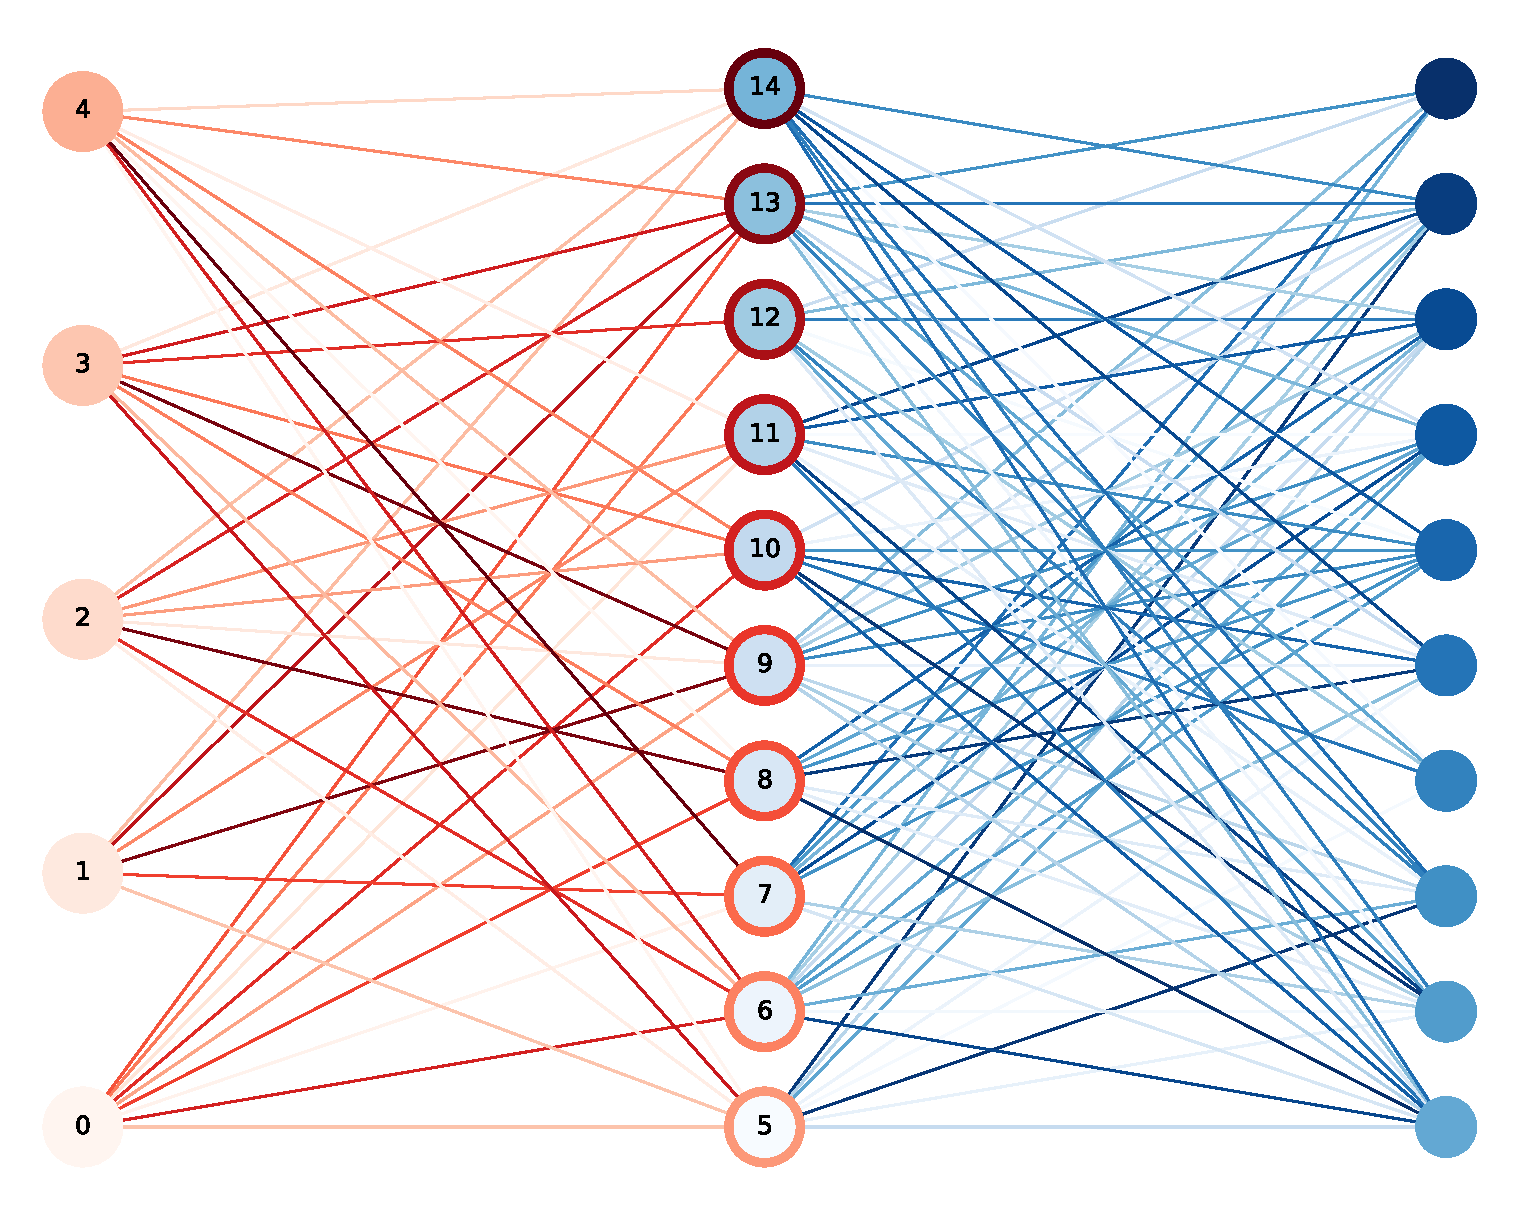
\includegraphics[width=0.45\textwidth]{FigureRobhoot.pdf}
  %\caption{
  {\small {\bf Figure 3: Robhoot in Digital Ecosystems}: {\bf Left
      column}: {\bf $\mathcal{ROBHOOT}$ v.1.0} representing the
    research cycle as nodes from number 0 to 4: Data integration (0),
    Complexity Reduction (1), Inference (2), Validation (3), and
    Visualization(4)). {\bf Central column}: Nodes representing the
    research cycle in the left column are connected to open-source
    software in the digital ecosystem. Connections with node number 0
    in the left column can, for example, represent the ETLs
    open-source software interactions required to generate the {\bf
      Universal ETLs} module. The same meaning applies to the
    different nodes of the left column. {\bf Right column}: Each node
    represents a report meaning there is a reporting gradient
    generated by the connections to the open-source software from
    where each report is generated only using a subset of the research
    layers and open-source software.}


\section{Their relevance in terms of Future and Emerging Technologies}

Table 2 


\subsection{Scientific concept}
Research cycle automation combining novel decentralization algorithms
with data, inference, and knowledge graphs integration

\subsection{Identified problem}
Global sustainability  is a major goal of humanity. Many studies have
shown global sustainability could be achieved by strengthening
transparency and feedbacks between social, ecological and governance
systems. Sustainability goals, however, strongly depend on global
society access to evidence- and research-based knowledge gaps. Yet,
the science ecosystem lacks open-source technologies narrowing down
the different aspects of knowledge gaps.


\subsection{Potential solutions envisaged}
\begin{itemize}
\item Global access to fully reproducible reports
\item Testnet case study in Sustainability and Biodiversity research to facilitate open an global access  
\end{itemize}

\subsection{Describe the vision of a radically-new science-enabled}


\subsection{Technology that the project would contribute towards}

\textcolor{red}{Implementation 3.1 Research methodology and work plan
  – Work packages, deliverables We will use a hybrid modular approach
  (refs for selecting project management) containing four objectives,
  eleven work packages and X deliverables. The following is the
  research methodology and timing of the work packages and the
  connections among the packages within and across goals: O1:
  Multilayer WP1 (ADAI): Automated data acquisition and
  integration. Open-source ETLs are rapidly evolving towards
  accounting for many key aspects of data integration: Data
  manipulation across formats (CloverDX), merging of historical and
  real-time streaming data pipelines (i.e., Kafka) and data structures
  facilitating the storage and access of large amounts of data (i.e.,
  clickhouse.) Our research methodology will be focused on developing
  an automated workflow using the geographically distributed cloud on
  computing and storage to test the robustness of data integration
  metrics across gradients of simulated data containing dimensions,
  biases, sizes, formats, temporal and spatial resolution (should we
  be more domain specific here? Or should we stay general and thinking
  broadly about simulated data with along complexity gradients and
  explore data integration metrics? How is the SDSC dealing with data
  integration for Renku?  MapReduce Golem network Resource
  distribution in data storage and simulating data (Ease.ml
  constraints and novelty and how Fluence network can help to solve
  it) WP2 (PROPANCE): Process pattern automated inference. Automated
  classification scheme to explore many inference methods across the
  population of KGs.  WP3 (VISUR): Intralayer visualization and
  reporting. We will integrate and develop new algorithms to merge
  distinct database into one large db using mySQL, clickhouse or
  similar db-open-source software.  WP4 (XX) Multilayer and KG
  integration: Existing knowledge of neural networks (refs by Luis)
  and deep knowledge-based algorithms to obtain the KGs (integrating
  WP1-3.)  automated ledger knowledge network technology to compactly
  facilitate open-science, decentralization, reproducibility and
  security in the science ecosystem O2: Ledger WP5 (): DeepKlen
  consensus protocol (DCP). The ledger represents the DeepKlen
  universe at a given point in time. It contains the KGs list and all
  the orders in the distributed network. We will define and implement
  a protocol to which KG set to apply to the last ledger. WP6 ():
  Scalability, decentralization and security protocols.  WP7 ():
  Ledger automation O3: DeepKlen WP8 (): Testnet WP9 (): Mainnet O4:
  Robhoot WP10 (): Testnet Showcase of the julia packages to be
  integrated within and between layers and the existing gaps. WP11 ():
  The Robhoot Open Network (RON) for Biodiversity research}

\subsection{Describe how this vision surpasses paradigms that
  currently exist}


\subsection{Overall and specific objectives for the project}
\textcolor{red}{High risk, plausibility and flexibility of the
  research approach\\ We are in need of accounting for the
  uncertainties, the reproducibility and immutability related to
  automation in science and engineering. This need is not just for a
  specific stage of the research cycle, but for the full research
  cycle, from data acquisition to reporting generation because
  knowledge-inspired societies and governance will demand full
  research cycle transparency in solving complex social, environmental
  and technological problems. This need brings many challenges to our
  research proposal because obtaining robust knowledge from
  integrating many parts each containing its own set of methods can
  generate divergent, fragile and contradictory outcomes. We will
  develop a flexible research method focusing more in the algorithmic
  robustness of the deep ledger knowledge network than in the
  development of robust automated knowledge generation. Our motivation
  will be to provide a first proof of concept of how the technology
  works: we will sample the KGs using different deep learning
  algorithms to estimate the uncertainty of the ruled-based inference
  obtained by fitting predictions to simulated data (Goal
  G1). Accounting for the uncertainties of each of the research stages
  when sampling the KGs comes from the many distinct paths within and
  across the layers in the research cycle (Figure 1). We will test a
  variety of consensus algorithms to explore the degree of security,
  decentralization and scalability of the ledger knowledge network
  using the generated population of KGs (Goal G2). Despite our focus
  will be bias towards the side of the algorithmic robustness of the
  deep ledger knowledge network, we will develop a domain-specific
  case study, our Robhoot Open Network, to test the robustness of the
  rule-based inference obtained by fitting each of the generated KG to
  the empirical patterns (Goal G3). The high risk associated to
  robustly automate the full research cycle for producing immutable
  open knowledge is buffered to a great extend because the existing
  ecosystem of tested and reliable open-source tools: We will combine
  our own algorithms (i.e., data integration and deep learning
  algorithms for sampling and automating the KGs) with open-source
  tools like Renku, Fabric and gitchain. This open-ecosystem will
  allow us to have a flexible launching of a testnet to collect data
  to explore the security-scalability-decentralization patterns and
  the robustness of the generated KGs in the deep ledger knowledge
  network (Goal G4.) }

\subsection{The relevant state-of-the-art and the extent of the
  advance the project would provide beyond it}

There are currently automated platforms mostly in the private domain
focusing in specific parts or one layer/one path of the research cycle
(BigQuery, Modulos, Google AI, Automated statistician; Ghahramani,
2015, Ease.ml; Li, Zhong, Liu, Wu, & Zhang, 2017)⁠: Novelty of
reporting generation following one path or resource allocation when
exploring many parts of the research cycle. The science ecosystem,
however, still lack a framework automating the research cycle from
end-to-end into the scalability-security-decentralization trade-offs
of digital ecosystems. Many science and engineering projects have
failed in reproducibility in public-funded science and technology
(refs). Yet, despite public institutions are demanding more
reproducibility and openness of the data and the scientific cycle
(refs), and overall a shifting towards open and reproducible
scientific and engineering landscapes, there are not currently open
technologies aiming to compactly facilitate and distribute the
scientific and engineering cycle in immutable knowledge networks.


\subsection{Science-to-technology breakthrough targeted by the
  project}
Closing global sustainability knowledge gaps in the science of bias in
neural spiking networks and automation in multilayer networks.


\subsection{Interdisciplinarity}
{\bf $\mathcal{ROBHOOT}$} aims to be a hybrid-technology accounting
for many features (Tables 1 to 3). Producing such a multi-feature
technology requires multidisciplinarity teams making contributions for
each of the Robhoot features while integrating all these features in a
rapidly evolving digital ecosystem. In this regard, the project aims
to put together data and computer scientists (i.e., distributed
computing, open-source software development), scientists from the
physics of complex systems (i.e., multilayer networks), artificial
intelligence (i.e., deep learning and automation) and the biology,
ecology and evolution of social, natural and technological ecosystems.

Technologies with the capacity to compactly account for neutral,
borderless, immutable, and open-access information in hybrid,
trusted-untrusted peer-to-peer interactions, accounting for the
multilayer nature of science and engineering are currently not in
place. Producing such a technology will require integrating expertise
from disparate disciplines like multilayer networks, deep learning,
automation algorithmics, and distributed technologies. The integration
of these disciplines will require to go beyond domain
boundaries. Specifically, we will merge scientists and engineers from
data and computer science, the physics of complex systems, artificial
intelligence and the biology, ecology and evolution of social, natural
and technological ecosystems to develop a “de novo” technology: the
synthesis of automated knowledge generation in a neutral, borderless
and immutable network synthesized anew from existing open-source
projects like Renku, Fabric and gitchain.


\subsection{Scientific and technological contributions to the
  foundation of a new future technology}

\textcolor{red}{Peer-to-peer interactions composed by trusting and
  untrusting peers abound in social, economical, natural and
  technological ecosystems. Many studies in such systems are producing
  an immense gain in detailed knowledge about scalability, security
  and decentralization trade-offs (refs; TON network; Fabric ledger OS
  network). Automation and AI technologies is the other angle from
  which many advances are rapidly occurring. While the existing
  technological paradigm is rapidly shifting towards science-based
  decentralization and automation technologies, end-to-end open-source
  research accounting for decentralized, neutral and automated
  knowledge-inspired technologies are missing. Most studies about
  these trade-offs have considered one-level networks. Yet,
  information generation usually comes from the interactions within-
  and between-layers, and the feedbacks occurring among layers in
  these systems have provided new unexpected behaviors that are
  difficult to anticipate when exploring one layer alone (refs). In
  biological systems, the genetic architecture of functionally
  important traits feedback throughout the genotype-phenotype map
  producing variation in phenotypes that are functionally important to
  understand the evolution of genotypic and phenotypic variation like
  growth rates and the immune system that ultimately determine the
  frequency of the phenotypes and the interaction centrality patterns
  in natural populations (refs). In science and engineering, many
  steps within- and between-layers occur to generate information
  (Figure 1a) Similarly to biological systems, interactions including
  intra- and inter-layer feedbacks are not easy to reproduce if not
  properly accounted for. One of the main facts when accounting for
  more than one layer is that the interactions and feedbacks to each
  other produce a dynamics that significantly differ from the
  one-layer approach (refs). Accounting for levels and scales in many
  systems using multilayer networks have provided a framework to
  explore how the microdynamics of peer-to-peer interactions might
  connect to the macroscopic properties of the ecosystem like the
  centralization and and the sensitivity to attacks within and between
  layers (refs).}

Science and technology ecosystems are in need of accounting for the
uncertainties, reproducibility and immutability related to the
complexity of the research process (Table 1). Such needs are not just
for a specific stage of the research cycle, but from data acquisition
and integration to automated reporting generation because
knowledge-inspired societies and decentralized governance will demand
full research cycle transparency to solve complex social,
environmental and technological problems (Tables 2 and 3). Reducing
knowledge-gaps at global scales in knowledge-inspired societies bring
many challenges to our research proposal because obtaining robust
knowledge from integrating many layers of the research cycle, each
containing its own set of methods and uncertainties, can generate
divergent, fragile and contradictory outcomes.

We will develop a flexible and adaptive research method focusing step
by step in increasing levels of complexity (i.e., from {\bf
  $\mathcal{ROBHOOT}$} v.1.0 to v.4.0, Figure 4). Our motivation will
be to provide a first open-access proof of concept of how the
technology works: we will automate reproducible research paths ({\bf
  $\mathcal{ROBHOOT}$} v.1.0) to sample the KGs ({\bf
  $\mathcal{ROBHOOT}$} v.2.0) contrasting deep learning algorithms to
estimate the uncertainty of the ruled-based inference obtained by
fitting predictions to simulated data ({\bf $\mathcal{ROBHOOT}$}
v.3.0). Accounting for the uncertainties of each of the research
stages when sampling the KGs comes from the many distinct paths within
and across the layers in the research cycle (Figure 2a). {\bf
  $\mathcal{ROBHOOT}$} v.4.0 will test a variety of consensus
algorithms to explore the degree of security, decentralization and
scalability of the ledger knowledge network using the generated
population of KGs.

Despite our focus will be bias towards the algorithmic robustness
during the four stages of development, we will implement a
domain-specific case study, a ``Biodiversity, Global Change and
Sustainability Research'', to test the robustness of the rule-based
inference obtained by fitting the KGs to empirical patterns. The high
risk associated to robustly automate the full research cycle for
producing immutable open knowledge will be buffered to a great extend
because the existing digital ecosystem of highly reliable open-source
software tools (Figure 3).
\begin{figure*}[ht]
  %\centering
  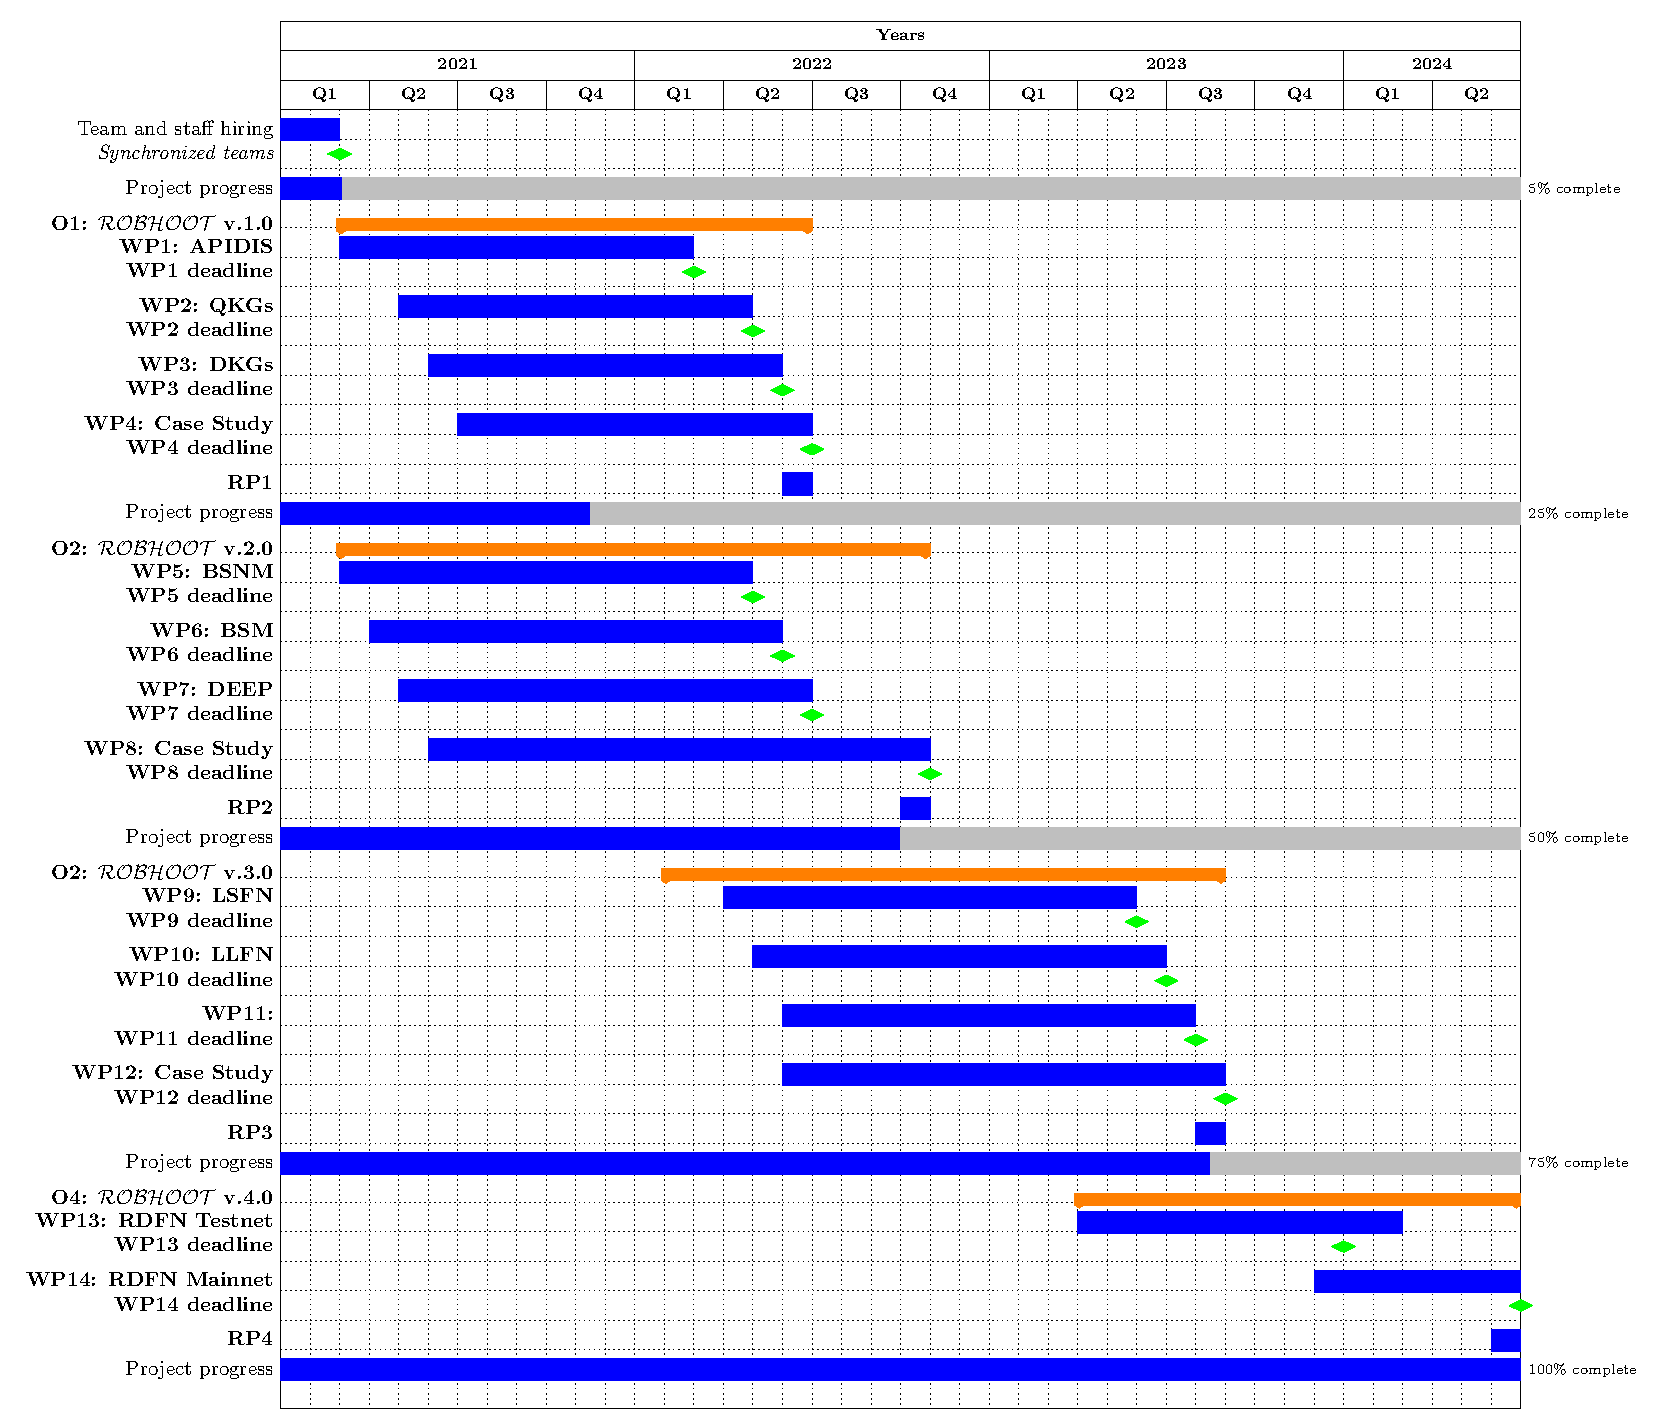
\includegraphics[width=1\textwidth]{GanttChart.pdf}
  {\small {\bf Figure 4: Roadmap}: {\bf $\mathcal{ROBHOOT}$ v.1.0}
    working packages {\bf WP1} to {\bf WP4} will take care of the
    integration of {\bf Universal ETLs}, {\bf Bayesian Space Models},
    {\bf Animation Space}, and {\bf Reporting} to automate fully the
    research cycle (Figure 2a). {\bf $\mathcal{ROBHOOT}$ v.2.0} {\bf
      WP5} to {\bf WP8} will deploy knowledge graphs (KGs) into a
    fully traceable research cycle (Figure 2b). {\bf
      $\mathcal{ROBHOOT}$ v.3.0} {\bf WP9} to {\bf WP12} will explore
    deep learning networks to sample KGs populations to gain
    understanding of the robustness of the patterns in the data under
    distinct research paths (Figure 2c). {\bf $\mathcal{ROBHOOT}$
      v.4.0} {\bf WP13} to {\bf WP16} will deploy KGs populations into
    a decentralized network of mutually trusting/untrusting peers with
    every peer maintaining the population of the KGs.}
\end{figure*}


\subsection{Potential for future social or economic impact or market
  creation}

The following are the general and the specific impacts according to
our objectives, working packages and deliverables:

\begin{itemize}
\item Automated knowledge-based network technology\\ The integration between open-source
data integration and inference schemes, the interlayer automation (O1:
Multilayer), will allow for the systematic exploration of robust
knowledge-based patterns when exploring the population of KGs. This is
in sharp contrast to existing AI technologies mostly oriented to
prediction without knowledge-based understanding (refs). Despite
open-source ETLs are rapidly evolving towards accounting for many
aspects of data integration (formats, historical-real time, storage,
dimensions, size, bias and spatiotemporal resolution), there is a
missing component in quantifying the robustness of knowledge that
integrated data can provide. Automated populations of KGs connecting
cutting-edge open-source ETLs to inference classification schemes can
provide the quantification of robustness in knowledge-based patters
for future predictive technologies.

\item Open immutable knowledge in untrusted digital peer-to-peer
  ecosystems\\
  The open access of immutable accumulation of knowledge in untrusted
  digital peer-to-peer ecosystems: Social, environmental and economic
  impact to facilitate global access to transparent knowledge.  ETLs
  are rapidly evolving towards accounting for many key aspects of data
  integration: Data manipulation across formats (CloverDX), merging of
  historical and real-time streaming data pipelines (i.e., Kafka) and
  data structures facilitating the storage and access of large amounts
  of data (i.e., clickhouse.) Our research methodology will be focused
  on developing an automated workflow using the geographically
  distributed cloud on computing and storage to test the robustness of
  data integration metrics across gradients of simulated data
  containing dimensions, biases, sizes, formats, temporal and spatial
  resolution (should we be more domain specific here? Or should we
  stay general and thinking broadly about simulated data with along
  complexity gradients and explore data integration metrics? How is
  the SDSC dealing with data integration for Renku?  We anticipate
  implementation of an automated end-to-end research cycle within an
  open ledger to facilitate real-time open-access neutral
  data-rule-knowledge to gain informed decisions to help solve complex
  social, environmental and technological problems. This facilitation
  might occur for local, regional and global problems in many
  fronts. Specifically, open deep ledger knowledge networks might have
  an impact in the following five areas

\item The identification of gaps in research paths not explored
  consequence of lack of synthesis in interdisciplinary research\\
  The creation of new markets opportunities obtained from exploring
  these gaps and the development of comparative method in the science
  of science and citizen data science.

  \item The merging of prediction
  and explanatory power in open science to gain synergy between AI
  open predictive tools and ruled-based pattern inference creating a
  more balanced pattern and process inference interaction. Recent
  examples of AI algorithms playing chess and go using brute force
  deep learning models or rule-based algorithms have discovered the
  power...: The integration between prediction and understanding power
  to facilitate explanatory synthesis.

\item The automation of reproducible open knowledge will facilitate
  the reusability, repeatability, and replicability of research
  outputs. The open access knowledge for governance transparency.

  \textcolor{red}{Measures to maximise impact a) Dissemination and
    exploitation of results 1. G4 will launch a testnet to help
    disseminate the main results of the deep ledger knowledge
    network. The launch will have invited NGO’s and GO across
    disciplines and social, economical and technological sectors.
    2. The Robhoot Open network will be launched as a Biodiversity
    research network to integrate the existing public databases and
    crowdsource data collections into the automated KGs and ledger
    network to facilitate NGOs, GO and other organizations
    transparency and governance in Biodiversity management. 3. The
    project aims to publish its main findings in top open scientific
    journals to communicate the global impact of a deep ledger
    knowledge network for transparency and governance across social
    and economical sectors. b) Communication activities 1. The
    contribution in communication of the Swiss Data Science Center,
    Switzerland 2. Contribution of the Wyss center 3. Contribution of
    Ifisc, Spain}

  
\subsection{Create new market opportunities, strengthen
  competitiveness and growth of companies, address issues related to
  climate change or the environment, or bring other important benefits
  for society}

\section{Impact}

\subsection{Expected impacts}


The following are the general and the specific impacts according to our objectives, working packages and deliverables:

\begin{itemize}
\item Automated knowledge-based network technology\\
  
  The integration between open-source data integration and inference
  schemes, the interlayer automation (O1: Multilayer), will allow for
  the systematic exploration of robust knowledge-based patterns when
  exploring the population of KGs. This is in sharp contrast to
  existing AI technologies mostly oriented to prediction without
  knowledge-based understanding (refs). Despite open-source ETLs are
  rapidly evolving towards accounting for many aspects of data
  integration (formats, historical-real time, storage, dimensions,
  size, bias and spatiotemporal resolution), there is a missing
  component in quantifying the robustness of knowledge that integrated
  data can provide. Automated populations of KGs connecting
  cutting-edge open-source ETLs to inference classification schemes
  can provide the quantification of robustness in knowledge-based
  patters for future predictive technologies.

\item Open immutable knowledge in untrusted digital peer-to-peer ecosystems\\
  
  The open access of immutable accumulation of knowledge in untrusted
  digital peer-to-peer ecosystems: Social, environmental and economic
  impact to facilitate global access to transparent knowledge.  ETLs
  are rapidly evolving towards accounting for many key aspects of data
  integration: Data manipulation across formats (CloverDX), merging of
  historical and real-time streaming data pipelines (i.e., Kafka) and
  data structures facilitating the storage and access of large amounts
  of data (i.e., clickhouse.) Our research methodology will be focused
  on developing an automated workflow using the geographically
  distributed cloud on computing and storage to test the robustness of
  data integration metrics across gradients of simulated data
  containing dimensions, biases, sizes, formats, temporal and spatial
  resolution (should we be more domain specific here? Or should we
  stay general and thinking broadly about simulated data with along
  complexity gradients and explore data integration metrics? How is
  the SDSC dealing with data integration for Renku?  We anticipate
  implementation of an automated end-to-end research cycle within an
  open ledger to facilitate real-time open-access neutral
  data-rule-knowledge to gain informed decisions to help solve complex
  social, environmental and technological problems. This facilitation
  might occur for local, regional and global problems in many
  fronts. Specifically, open deep ledger knowledge networks might have
  an impact in the following five areas
  
\item The identification of gaps in research paths not explored
  consequence of lack of synthesis in interdisciplinary research: The
  creation of new markets opportunities obtained from exploring these
  gaps and the development of comparative method in the science of
  science and citizen data science.

\item The merging of prediction and explanatory power in open science
  to gain synergy between AI open predictive tools and ruled-based
  pattern inference creating a more balanced pattern and process
  inference interaction. Recent examples of AI algorithms playing
  chess and go using brute force deep learning models or rule-based
  algorithms have discovered the power...: The integration between
  prediction and understanding power to facilitate explanatory
  synthesis.

\item The automation of reproducible open knowledge will facilitate
  the reusability, repeatability, and replicability of research
  outputs. The open access knowledge for governance transparency.

\subsection{Measures to maximise impact}

  \begin{itemize}
  \item Dissemination and exploitation of results

    1. G4 will launch a testnet to help disseminate the main results
    of the deep ledger knowledge network. The launch will have invited
    NGO’s and GO across disciplines and social, economical and
    technological sectors.

    2. The Robhoot Open network will be launched as a Biodiversity
    research network to integrate the existing public databases and
    crowdsource data collections into the automated KGs and ledger
    network to facilitate NGOs, GO and other organizations
    transparency and governance in Biodiversity management.

    3. The project aims to publish its main findings in top open
    scientific journals to communicate the global impact of a deep
    ledger knowledge network for transparency and governance across
    social and economical sectors.

\item Communication activities

  1. The contribution in communication of the Swiss Data Science Center, Switzerland

  2. Contribution of the Wyss center

  3. Contribution of Ifisc, Spain

\section{Implementation}

\subsection{Research methodology and work plan – Work packages,
  deliverables}

  \textcolor{red}{3. Implementation 3.1 Research methodology and work
    plan – Work packages, deliverables We will use a hybrid modular
    approach (refs for selecting project management) containing four
    objectives, eleven work packages and X deliverables. The following
    is the research methodology and timing of the work packages and
    the connections among the packages within and across goals: O1:
    Multilayer WP1 (ADAI): Automated data acquisition and
    integration. Open-source ETLs are rapidly evolving towards
    accounting for many key aspects of data integration: Data
    manipulation across formats (CloverDX), merging of historical and
    real-time streaming data pipelines (i.e., Kafka) and data
    structures facilitating the storage and access of large amounts of
    data (i.e., clickhouse.) Our research methodology will be focused
    on developing an automated workflow using the geographically
    distributed cloud on computing and storage to test the robustness
    of data integration metrics across gradients of simulated data
    containing dimensions, biases, sizes, formats, temporal and
    spatial resolution (should we be more domain specific here? Or
    should we stay general and thinking broadly about simulated data
    with along complexity gradients and explore data integration
    metrics? How is the SDSC dealing with data integration for Renku?
    MapReduce Golem network Resource distribution in data storage and
    simulating data (Ease.ml constraints and novelty and how Fluence
    network can help to solve it) WP2 (PROPANCE): Process pattern
    automated inference. Automated classification scheme to explore
    many inference methods across the population of KGs.  WP3 (VISUR):
    Intralayer visualization and reporting. We will integrate and
    develop new algorithms to merge distinct database into one large
    db using mySQL, clickhouse or similar db-open-source software.
    WP4 (XX) Multilayer and KG integration: Existing knowledge of
    neural networks (refs by Luis) and deep knowledge-based algorithms
    to obtain the KGs (integrating WP1-3.)  automated ledger knowledge
    network technology to compactly facilitate open-science,
    decentralization, reproducibility and security in the science
    ecosystem O2: Ledger WP5 (): DeepKlen consensus protocol (DCP).
    The ledger represents the DeepKlen universe at a given point in
    time. It contains the KGs list and all the orders in the
    distributed network. We will define and implement a protocol to
    which KG set to apply to the last ledger.  WP6 (): Scalability,
    decentralization and security protocols.  WP7 (): Ledger
    automation O3: DeepKlen WP8 (): Testnet WP9 (): Mainnet O4:
    Robhoot WP10 (): Testnet Showcase of the julia packages to be
    integrated within and between layers and the existing gaps.  WP11
    (): The Robhoot Open Network (RON) for Biodiversity research}

  \subsection{Management structure, milestones and procedures}
  \begin{itemize}
  \item Describe the organisational structure and the decision-making
    (including a list of milestones (table 3.2a))
  \item Explain why the organisational structure and decision-making
    mechanisms are appropriate to the complexity and scale of the
    project.
  \item Describe any critical risks, relating to project
    implementation, that the stated project's objectives may not be
    achieved. Detail any risk mitigation measures. Please provide a
    table with critical risks identified and mitigating actions (table
    3.2b) and relate these to the milestones.
  \end{itemize}

  \subsection{Consortium as a whole}

  \textcolor{red}{The individual members of the consortium are
    described in a separate section 4. There is no need to repeat that
    information here.  • Describe the consortium. Explain how it will
    support achieving the project objectives.  Does the consortium
    provide all the necessary expertise? Is the interdisciplinarity in
    the breakthrough idea reflected in the expertise of the
    consortium?  • In what way does each of the partners contribute to
    the project? Show that each has a valid role and adequate
    resources in the project to fulfil that role. How do the members
    complement one another?  Other countries and international
    organisations: If one or more of the participants requesting EU
    funding is based in a country or is an international organisation
    that is not automatically eligible for such funding (entities from
    Member States of the EU, from Associated Countries and from one of
    the countries in the exhaustive list included in General Annex A
    of the work programme are automatically eligible for EU funding),
    explain why the participation of the entity in question is
    considered essential for carrying out the action on the grounds
    that participation by the applicant has clear benefits for the
    consortium.}


  \subsection{Resources to be committed}

  \textcolor{red}{Please make sure the information in this section
    matches the costs as stated in the budget table in section 3 of
    the administrative proposal forms, and the number of person
    months, shown in the detailed work package descriptions.  Please
    provide the following: • a table showing number of person months
    required (table 3.4a) • a table showing ‘other direct costs’
    (table 3.4b) for participants where those costs exceed 15\% of the
    personnel costs (according to the budget table in section 3 of the
    administrative proposal forms)}
  
%----------------------------------------------------------------------------------------
%	BIBLIOGRAPHY
%----------------------------------------------------------------------------------------

%\printbibliography[title={Bibliography}] % Print the bibliography, section title in curly brackets

\newpage
\bibliographystyle{unsrtnat}
%\bibliographystyle{tree.bst}
\bibliography{Robhoot.bib}

%----------------------------------------------------------------------------------------

\end{document}

\hspace{-0.2 in}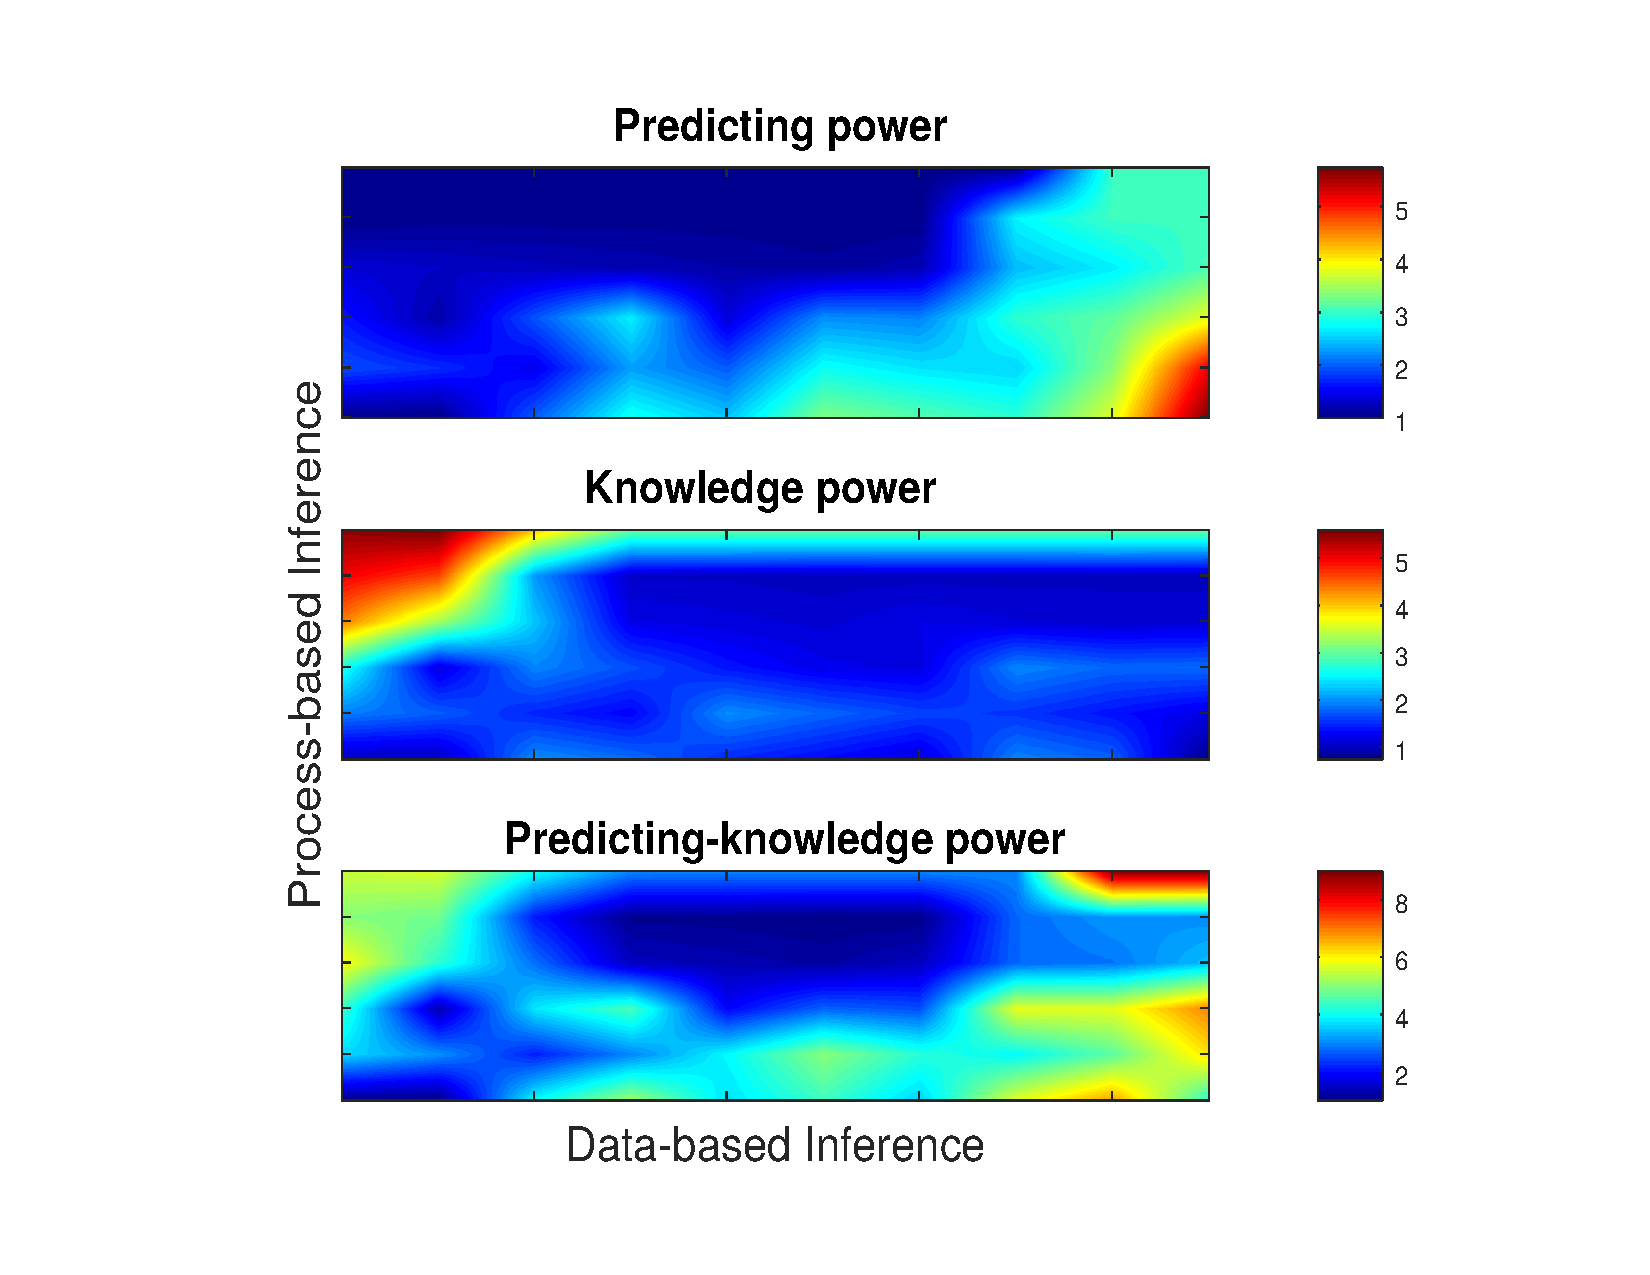
\includegraphics[width=0.52\textwidth]{Figure3.pdf}
{\small {\bf Figure 1: Prediction power (top), understanding (middle),
    and prediction-understanding power maps (bottom)}. x-axis
  represents data-based inference (i.e., gradient of AI methods from
  low (left) to high (right) predictive power). y-axis represents
  process-based inference (i.e., gradient of process-based methods
  from low (bottom left) to high (top left) understanding power). The
  gradient of predicting power map (top) shows a hot spot red area in
  the bottom right highlighting the region where AI methods best
  predict the empirical data. The gradient of understanding power map
  (middle) shows a red hot spot in the top left highlighting the
  region where the best mechanistic understanding occur. The
  predicting-understanding power map (bottom) shows the sum of the two
  previous maps highlighting a red hot spot where the best synthesis
  research joining predicting and understanding power of the empirical
  data might occur. The first research goal of this proposal aims to
  build an automated research platform to maximize the predicting and
  understanding power highlighted in the red hot spot of the
  predicting-understanding power map (bottom).}
